%% LaTeX2e class for student theses
%% thesis.tex
%% 
%% Karlsruhe Institute of Technology
%% Institute for Program Structures and Data Organization
%% Chair for Software Design and Quality (SDQ)
%%
%% Dr.-Ing. Erik Burger
%% burger@kit.edu
%%
%% Version 1.3.3, 2018-04-17

%% Available page modes: oneside, twoside
%% Available languages: english, ngerman
%% Available modes: draft, final (see README)
\documentclass[twoside, english, final]{sdqthesis}

%% ---------------------------------
%% | Information about the thesis  |
%% ---------------------------------

%% Name of the author
\author{Lucas Werkmeister}

%% Title (and possibly subtitle) of the thesis
\title{Schema Inference on Wikidata}

%% Type of the thesis 
\thesistype{Master's Thesis}

%% Change the institute here, ``IPD'' is default
% \myinstitute{Institute for \dots}

%% You can put a logo in the ``logos'' directory and include it here
%% instead of the SDQ logo
% \grouplogo{myfile}
%% Alternatively, you can disable the group logo
% \nogrouplogo

%% The reviewers are the professors that grade your thesis
\reviewerone{Prof. Reussner}
\reviewertwo{Prof. Sack}

%% The advisors are PhDs or Postdocs
\advisorone{Dr. Koutraki}

%% Please enter the start end end time of your thesis
\editingtime{16. April 2018}{15. October 2018}

\settitle

%% --------------------------------
%% | Settings for word separation |
%% --------------------------------

%% Describe separation hints here.
%% For more details, see 
%% http://en.wikibooks.org/wiki/LaTeX/Text_Formatting#Hyphenation
\hyphenation{
% me-ta-mo-del
}

%% --------------------------------
%% | Bibliography                 |
%% --------------------------------

%% Use biber instead of BibTeX, see README
\usepackage[citestyle=numeric,style=numeric,backend=biber]{biblatex}
\addbibresource{thesis.bib}

%% --------------------------------
%% | Glossary                     |
%% --------------------------------

\usepackage{glossaries}
\makeglossaries
% TODO define terms for Label, Description, Statement, etc.,
% then write them all in uppercase per Lydia’s comment
\newacronym{imdb}{IMDb}{Internet Movie Database}
\newacronym{loc}{LoC}{Library of Congress}
\newacronym{rdf}{RDF}{Resource Description Framework}
\newacronym[longplural={Requests for Comments}]{rfc}{RfC}{Request for Comments}
\newacronym{shex}{ShEx}{Shape Expressions}
\newacronym{sparql}{SPARQL}{SPARQL Protocol and RDF Query Language}
\newacronym[first={the Virtual International Authority File},long={the Virtual International Authority File}]{viaf}{VIAF}{Virtual International Authority File}
\newacronym{w3c}{W3C}{World Wide Web Consortium}
\newacronym[first={the Wikidata Query Service},long={the Wikidata Query Service}]{wdqs}{WDQS}{Wikidata Query Service}
\newacronym[description={Internationalized Resource Identifier, Unicode-aware generalization of \glspl{uri}}]{iri}{IRI}{Internationalized Resource Identifier}
\newacronym[description={Uniform Resource Identifier, usually a \gls{url}}]{uri}{URI}{Uniform Resource Identifier}
\newacronym{url}{URL}{Uniform Resource Locator}
\newacronym{html}{HTML}{Hypertext Markup Language}
\newacronym{css}{CSS}{Cascading Style Sheets}
\newacronym{http}{HTTP}{Hypertext Transfer Protocol}

% never use the long form of these acronyms unless explicitly requested
\glsunset{url}
\glsunset{html}
\glsunset{css}
\glsunset{http}

\newglossaryentry{Wikimedia}{
  name=Wikimedia,
  description={free knowledge movement and community},
}
\newglossaryentry{Wikidata}{
  name=Wikidata,
  description={free knowledge base in the \gls{Wikimedia} movement},
}
\newglossaryentry{Wikipedia}{
  name=Wikipedia,
  description={free encyclopedia in the \gls{Wikimedia} movement},
}
\newglossaryentry{Wikimedia Commons}{
  name={Wikimedia Commons},
  description={free media repository in the \gls{Wikimedia} movement},
}
\newglossaryentry{Wikiquote}{
  name=Wikiquote,
  description={free quotation collection in the \gls{Wikimedia} movement},
}
\newglossaryentry{item}{
  name=item,
  description={representation of a thing or concept in \gls{Wikidata}},
}
\newglossaryentry{item ID}{
  name={item ID},
  description={unique, language-agnostic identifier of an \gls{item}, a consecutive number prefixed with the letter “Q”},
}
\newglossaryentry{property}{
  name=property,
  plural=properties,
  description={a possible feature, characteristic or quality of an \gls{item}},
}
\newglossaryentry{property ID}{
  name={property ID},
  description={unique, language-agnostic identifier of a \gls{property}, a consecutive number prefixed with the letter “P”},
}
\newglossaryentry{label}{
  name=label,
  description={the primary term for an \gls{item} or \gls{property} in a language},
}
\newglossaryentry{description}{
  name=description,
  description={a short clarifying or disambiguating text for an \gls{item} or \gls{property}},
}
\newglossaryentry{alias}{
  name=alias,
  plural=aliases,
  description={additional terms by which an \gls{item} or \gls{property} should be found},
}
\newglossaryentry{sitelink}{
  name=sitelink,
  description={a link from an \gls{item} to a page in a \gls{Wikimedia} project about the thing or concept the \gls{item} represents},
}
\newglossaryentry{statement}{
  name=statement,
  description={a unit of information in \gls{Wikidata}, consisting of a subject \gls{item}, a predicate \gls{property}, and a value (\gls{item ID}, quantity, point in time, etc.)},
}
\newglossaryentry{qualifier}{
  name=qualifier,
  description={an additional \gls{property}-value pair further refining a \gls{statement}},
}
\newglossaryentry{reference}{
  name=reference,
  description={a collection of \gls{property}-value pairs recording a source for a \gls{statement}},
}
\newglossaryentry{wdsi}{
  name={Wikidata Shape Expressions Inference tool},
  description={web-based tool to make the inference process available to the \gls{Wikidata} community},
}
\newglossaryentry{triple}{
  name=triple,
  description={a unit of information in \gls{rdf}, consisting of a \gls{subject} \gls{resource}, a \gls{predicate} \gls{resource}, and an \gls{object} value (\gls{resource} or literal)},
}
\newglossaryentry{subject}{
  name=subject,
  description={the first element of an \gls{rdf} \gls{triple}, the “<Alan Turing>” in “<Alan Turing> <is a> <human>”}
}
\newglossaryentry{predicate}{
  name=predicate,
  description={the second element of an \gls{rdf} \gls{triple}, the “<is a>” in “<Alan Turing> <is a> <human>”}
}
\newglossaryentry{object}{
  name=object,
  description={the third element of an \gls{rdf} \gls{triple}, the “<human>” in “<Alan Turing> <is a> <human>”}
}
\newglossaryentry{resource}{
  name=resource,
  description={representation of a thing or concept in \gls{rdf}, identified by an \gls{iri}},
}
\newglossaryentry{schema}{
  name=schema,
  description={formal description of the structure of a linked data set; in \gls{shex}, a collection of \glspl{shape}},
}
\newglossaryentry{shape}{
  name=shape,
  description={element of a \gls{shex} \gls{schema}, describing the structure of one node category},
}
\newglossaryentry{RDF2Graph}{
  name={RDF\oldstylenums{2}Graph},
  description={tool to automatically determine a \gls{schema} from an \gls{rdf} graph},
}
\newglossaryentry{RDFSimpleCon}{
  name=RDFSimpleCon,
  description={library used by \gls{RDF2Graph}},
}


%% --------------------------------
%% | Listings                     |
%% --------------------------------

% https://tex.stackexchange.com/a/279245/25264
\usepackage{float}
\usepackage{subcaption}
\usepackage{listings}
\usepackage{cleveref}
\newfloat{lstfloat}{htbp}{lop} % TODO I’m not sure about that placement, perhaps just tbp (top, bottom, own page)?
\floatname{lstfloat}{Listing}
\crefalias{lstfloat}{listing}
\lstset{
  basicstyle=\ttfamily,
}

%% --------------------------------
%% | Macros                       |
%% --------------------------------

\newcommand{\Q}[1]{\href{http://www.wikidata.org/entity/#1}{#1}}
\renewcommand{\P}[1]{\href{http://www.wikidata.org/entity/#1}{#1}}
\newcommand{\PName}[1]{\texttt{#1}}

%% ====================================
%% ====================================
%% ||                                ||
%% || Beginning of the main document ||
%% ||                                ||
%% ====================================
%% ====================================
\begin{document}

%% Set PDF metadata
\setpdf

%% Set the title
\maketitle

%% The Preamble begins here
\frontmatter

%% LaTeX2e class for student theses: Declaration of independent work
%% sections/declaration.tex
%% 
%% Karlsruhe Institute of Technology
%% Institute for Program Structures and Data Organization
%% Chair for Software Design and Quality (SDQ)
%%
%% Dr.-Ing. Erik Burger
%% burger@kit.edu
%%
%% Version 1.3.3, 2018-04-17

\thispagestyle{empty}
\null\vfill
\noindent\hbox to \textwidth{\hrulefill} 
\iflanguage{english}{I declare that I have developed and written the enclosed
thesis completely by myself, and have not used sources or means without
declaration in the text.}%
{Ich versichere wahrheitsgemäß, die Arbeit
selbstständig angefertigt, alle benutzten Hilfsmittel vollständig und genau
angegeben und alles kenntlich gemacht zu haben, was aus Arbeiten anderer
unverändert oder mit Änderungen entnommen wurde.}
 
 
%% ---------------------------------------------
%% | Replace PLACE and DATE with actual values |
%% ---------------------------------------------
\textbf{PLACE, DATE}
\vspace{1.5cm}
 
\dotfill\hspace*{8.0cm}\\
\hspace*{2cm}(\theauthor) 
\cleardoublepage

\setcounter{page}{1}
\pagenumbering{roman}

%% ----------------
%% |   Abstract   |
%% ----------------
 
%% For theses written in English, an abstract both in English
%% and German is mandatory.
%%
%% For theses written in German, a German abstract is sufficient.
%%
%% The text is included from the following files:
%% - sections/abstract

\includeabstract

%% ------------------------
%% |   Table of Contents  |
%% ------------------------
\tableofcontents

\listoffigures
\listoftables

%% -----------------
%% |   Main part   |
%% -----------------

\mainmatter

%% LaTeX2e class for student theses
%% sections/content.tex
%% 
%% Karlsruhe Institute of Technology
%% Institute for Program Structures and Data Organization
%% Chair for Software Design and Quality (SDQ)
%%
%% Dr.-Ing. Erik Burger
%% burger@kit.edu
%%
%% Version 1.3.3, 2018-04-17

\chapter{Introduction}
\label{ch:Introduction}

Data quality has been identified as one of the most important areas of development for Wikidata in the future \cite{wdcon2017-sotp}: % TODO \cite before colon looks ugly
in order for Wikidata to be useful,
its data must be trustworthy and available in a consistent format.
Unchecked vandalism discourages data reuse,
while inconsistent data models make it significantly more difficult or even impossible.

To combat these problems,
several quality control mechanisms are used on Wikidata.
Recently, editors have begun exploring the use of \acrlong{shex}
as another quality control mechanism to use.
Compared to the more established, Wikidata-specific quality constraints system,
\acrlong{shex} are more powerful and expressive,
and are also not specific to Wikidata alone.
However, schemas for \acrlong{shex} are tedious to write by hand.

Automatically inferring schemas from Wikidata items
promises to simplify the schema authoring process:
instead of manually putting together the schema,
describing shapes for different classes of items,
one simply selects a set of items,
and a schema is automatically generated based on the data about these items.
If the selected items have been carefully edited
to conform to a pre-existing schema,
perhaps described informally or only present in the minds of the editors,
then the result may be a formalization of that schema;
alternatively, applying the same process to a less curated set of input items
may result in a concise summary of the current schema of those items % TODO “concise” is not really the right word…
and possibly even demonstrate problems in the input data.

% TODO probably mention WikiProject ShEx?

%% LaTeX2e class for student theses
%% sections/content.tex
%% 
%% Karlsruhe Institute of Technology
%% Institute for Program Structures and Data Organization
%% Chair for Software Design and Quality (SDQ)
%%
%% Dr.-Ing. Erik Burger
%% burger@kit.edu
%%
%% Version 1.3.3, 2018-04-17

\chapter{Background}
\label{ch:Background}

This chapter provides background information
on several concepts that are important to the rest of this thesis.
The sections below are not intended to be comprehensive introductions to the respective topics,
but focus on the aspects that are necessary to understand the thesis,
omitting parts that are unnecessary or distracting in this context.
Further information, including full introductions to most topics covered here,
can be found in the works listed in the bibliography.

\section{RDF}
\label{sec:Background:RDF}

\acrfull{rdf}
\cite{Lanthaler:14:RCA}
is a framework for describing and working with \gls{Linked Data},
developed by the \gls{rdf} Working Group under the umbrella of the \gls{w3c}.
In \gls{rdf}, information is arranged in \gls{subject}-\gls{predicate}-\gls{object} \glspl{triple},
such as “<Alan Turing> <is a> <human>”
or “<Lima> <was founded in> <18 January 1535>”.
All three elements of a \gls{triple} are typically \glspl{resource},
identified by an \gls{iri} like \url{http://example.com/Alan_Turing} or \url{http://www.wikidata.org/entity/Q5},
but the \gls{object} of a \gls{triple} can also be some other kind of value,
such as a textual, numerical or other literal
(e.~g. the date literal “18 January 1535” above).
A collection of such \glspl{triple} forms a directed, labeled graph,
where the \glspl{triple} describe individual edges
and the nodes are the \glspl{subject} and \glspl{object} of the \glspl{triple}:
\glspl{triple} with the same \gls{subject} constitute different outgoing arcs from the same node.
This graph can then be queried using the \acrfull{sparql} \cite{9569543}.
For a more detailed introduction to \gls{rdf} and related technologies,
see the RDF 1.1 Primer \cite{Schreiber:14:RP}.

To improve readability, the \glspl{iri} identifying a \gls{resource}
are usually abbreviated using \glspl{prefix}.
For example, once the \gls{prefix} \prefix{ex:} has been defined to mean \url{http://shex.example/},
the \glspl{iri} \url{http://shex.example/Person} and \url{http://shex.example/dateOfBirth}
can be abbreviated as \PName{ex:Person} and \PName{ex:dateOfBirth}.
(This “example” \gls{prefix}, also used below for other examples,
follows the naming conventions of schema.org \cite{schema.org-old-extension},
in that types (\PName{ex:Person}) and entities (\PName{ex:JohnDoe}) are in upper camel case
while predicates (\PName{ex:dateOfBirth}) are in lower camel case.)

While \gls{rdf} can be used with any \gls{resource} \glspl{iri},
one of its strengths is the ability to reuse the same \emph{vocabularies}
(effectively, sets of \glspl{resource})
in many different graphs.
For example, many graphs use the same \gls{predicate}, \PName{rdfs:label},
to link a \gls{resource} to a human-readable version of its name (its label);
a tool based on \gls{rdf} can thus offer human-readable names for \glspl{resource} from all these graphs
without requiring any specific knowledge about them,
and the graphs are more useful when used in combination.
One common vocabulary is \acrfull{rdfs} \cite{Guha:14:RS},
which among others provides two important predicates:
\PName{rdf:type} and \PName{rdfs:subClassOf}.
\PName{rdf:type} connects an object to its class,
and \PName{rdfs:subClassOf} connects a class to its parent class.
(The \prefix{rdf:} and \prefix{rdfs:} \glspl{prefix} are both part of \acrlong{rdfs};
the distinction between them is “a somewhat annoying historical artifact” \cite{Schreiber:14:RP}
with no real significance today.)
Another commonly used vocabulary is \gls{xsd} \cite{Malhotra:04:XSP},
which provides several basic datatypes:
for example, \PName{xsd:string} is the datatype for a simple text string (language-agnostic),
and \PName{xsd:date} and \PName{xsd:dateTime} are used to notate points in time.

\Cref{fig:rdf-example} shows a small example \gls{rdf} graph
for President Franklin D.~ Roosevelt and his pet dog, Fala.
The nodes with rounded corners represent \glspl{resource},
whereas the nodes with pointed corners are literals,
with their datatype given below them in parentheses.
Each arrow denotes a \gls{triple}, pointing from the \gls{subject} to the \gls{object},
with the \gls{predicate} written next to the arrow.
The graph describes the name and date of birth of the president and his dog,
their ownership relation,
and their types, including subtype relations:
Franklin D.~Roosevelt is a person, Fala is a dog,
and both persons and dogs are kinds of creatures.

The same graph may also be written textually in several syntaxes.
The simplest \gls{rdf} syntax is \gls{N-Triples} \cite{Seaborne:14:RN},
which lists \glspl{triple} one per line, each terminated with a period.
\Glspl{iri} are enclosed in angle brackets,
and literals are enclosed in double quotes,
optionally followed by two carets and their datatype
(otherwise the implied datatype is \PName{xsd:string}).
The \gls{N-Triples} representation of the same graph as in \cref{fig:rdf-example}
is presented in \cref{lst:rdf-example};
since \gls{N-Triples} does not allow the use of \glspl{prefix} to abbreviate \glspl{iri},
the \namecref{lst:rdf-example} has been rotated to fit the full width on the page.

\begin{figure}
  \centering
  \begin{tikzpicture}
    \tikzstyle{resource} = [rectangle, draw, rounded corners, text centered]
    \tikzstyle{literal} = [draw, text centered]
    \tikzstyle{arrow} = [draw, -latex']

    \begin{scope}
      \node[resource] (Creature) {\PName{ex:Creature}};
      \node[resource, below left=1cm and 1.5cm of Creature] (Human) {\PName{ex:Human}};
      \node[resource, below right=1cm and 1.5cm of Creature] (Dog) {\PName{ex:Dog}};
      \node[resource, below=1cm of Human] (FDR) {\PName{ex:FDR}};
      \node[resource, below=1cm of Dog] (Fala) {\PName{ex:Fala}};
    \end{scope}
    \begin{scope}[node distance=3cm, every text node part/.style={align=center}]
      \node[literal, below left of=FDR] (FDRDOB) {\graphRdfLiteral{1882-01-30}{xsd:date}};
      \node[literal, below of=FDR, node distance=4cm] (FDRName) {\graphRdfLiteral{Franklin Delano Roosevelt}{xsd:string}};
      \node[literal, below left of=Fala] (FalaName) {\graphRdfLiteral{Fala}{xsd:string}};
      \node[literal, below right of=Fala] (FalaDOB) {\graphRdfLiteral{1940-04-07}{xsd:date}};
    \end{scope}

    \begin{scope}[every path/.style=arrow, midway, auto]
      \path[left] (Human) -- node {\PName{rdfs:subClassOf}} (Creature);
      \path[right] (Dog) -- node {\PName{rdfs:subClassOf}} (Creature);
      \path[left] (FDR) -- node {\PName{rdf:type}} (Human);
      \path[right] (Fala) -- node {\PName{rdf:type}} (Dog);
      \path (FDR.north east) -- node {\PName{ex:pet}} (Fala.north west);
      \path (Fala.south west) -- node {\PName{ex:owner}} (FDR.south east);
      \path[left] (FDR) -- node {\PName{ex:dateOfBirth}} (FDRDOB);
      \path[right] (FDR) -- node {\PName{rdfs:label}} (FDRName);
      \path[left] (Fala) -- node {\PName{rdfs:label}} (FalaName);
      \path[right] (Fala) -- node {\PName{ex:dateOfBirth}} (FalaDOB);
    \end{scope}
  \end{tikzpicture}
  \caption{An \gls{rdf} graph for President Franklin D.~Roosevelt and his dog.}
  \label{fig:rdf-example}
\end{figure}

\begin{sidewayslstfloat}
\begin{lstlisting}
<http://shex.example/FDR> <http://www.w3.org/1999/02/22-rdf-syntax-ns#type> <http://shex.example/Human>.
<http://shex.example/FDR> <http://www.w3.org/2000/01/rdf-schema#label> "Franklin Delano Roosevelt".
<http://shex.example/FDR> <http://shex.example/dateOfBirth> "1882-01-30"^^<http://www.w3.org/2001/XMLSchema#date>.
<http://shex.example/FDR> <http://shex.example/pet> <http://shex.example/Fala>.
<http://shex.example/Fala> <http://www.w3.org/1999/02/22-rdf-syntax-ns#type> <http://shex.example/Dog>.
<http://shex.example/Fala> <http://www.w3.org/2000/01/rdf-schema#label> "Fala".
<http://shex.example/Fala> <http://shex.example/dateOfBirth> "1940-04-07"^^<http://www.w3.org/2001/XMLSchema#date>.
<http://shex.example/Fala> <http://shex.example/owner> <http://shex.example/FDR>.
<http://shex.example/Human> <http://www.w3.org/2000/01/rdf-schema#subClassOf> <http://shex.example/Creature>.
<http://shex.example/Dog> <http://www.w3.org/2000/01/rdf-schema#subClassOf> <http://shex.example/Creature>.
\end{lstlisting}
\caption{An \gls{rdf} graph for President Franklin D.~Roosevelt and his dog.}
\label{lst:rdf-example}
\end{sidewayslstfloat}

\section{Wikidata}
\label{sec:Background:Wikidata}

\Gls{Wikidata} \cite{Vrandecic:2014:WFC:2661061.2629489}
is a free knowledge base
and part of the \gls{Wikimedia} family of projects,
the most famous of which is \gls{Wikipedia}, the free encyclopedia.
Its contents are created, maintained and managed by the \gls{Wikidata} community,
most of whose members are volunteers,
as well as the members of other \gls{Wikimedia} projects, e.~g. \gls{Wikipedia}.
Anyone can contribute to \gls{Wikidata},
but the community ensures the quality of the contents with various quality control mechanisms.
Providing another such mechanism is part of the motivation for this thesis.

Information on \gls{Wikidata} is collected in \glspl{item},
which represent things or concepts:
there are \glspl{item} for individual persons,
for cities, states, geographical features,
for organizations and corporations,
\glspl{item} for books, films, newspapers, journals, scientific articles,
for abstract concepts, phenomena, emotions, philosophical movements, political orientations,
\glspl{item} for conceptual hierarchies, parent classes, biological taxa,
and even \glspl{item} for fictional characters, places, or other entities.

All of these \glspl{item} follow the same structure.
They are identified by their \gls{item ID},
a consecutive number prefixed with the letter “Q”
(e.~g. \Q{Q188709} for Beethoven’s Symphony No. 5).
They can have a \gls{label}, a \gls{description}, and \glspl{alias}, each in various languages:
for example, the \gls{item} \Q{Q7251} is labeled “Alan Turing” in English
but «\foreignlanguage{russian}{Алан Тьюринг}» in Russian;
is described as a “British mathematician, logician, cryptanalyst, and computer scientist” in English;
and may also be found under search aliases like “Alan M. Turing”, “Alan Mathison Turing” or simply “Turing”.
\Glspl{item} also have a set of \glspl{sitelink}
(links to pages about the same concept in various other \gls{Wikimedia} projects –
\gls{Wikipedia} articles, \gls{Wikiquote} pages, \gls{Wikimedia Commons} galleries, etc.),
and most importantly, a set of \glspl{statement}.

The \glspl{statement} are where most of the information in \gls{Wikidata} is stored.
They consist of a \gls{property}, such as “place of birth” or “author” or “population”,
and a value, which can be a reference to another \gls{item}, a quantity, a point in time, a piece of text,
or a few other possible types.
A \gls{statement} can also have \glspl{qualifier}
(further property-value pairs, e.~g. clarifying when or where the statement is valid)
and \glspl{reference} (sets of property-value pairs, listing sources for the \gls{statement}),
but those are mostly ignored in the context of this thesis.
\Glspl{property} are also identified by an ID, their \gls{property ID}
(prefixed with the letter “P” instead of “Q”),
and can also have \glspl{label}, \glspl{description} and \glspl{alias} in different languages:
for example, \P{P31} is labeled “instance of” in English
and „\foreignlanguage{ngerman}{ist ein(e)}“ in German.
The \glspl{label} and \glspl{description} are necessary to understand the meaning of \glspl{statement},
but they are not themselves part of the \glspl{statement}:
\glspl{statement} only list references to \gls{property} and \glspl{item ID},
making most of the information in \gls{Wikidata} language-agnostic \cite{Kaffee:2017:GBA:3125433.3125465}.

\Cref{fig:montblanc} shows two screenshots of the same \gls{Wikidata} \gls{item},
\QL{Q761735}{Montblanc}, viewed in different languages,
both as of \wikidataPermalink{704641959}.
The page structure is the same regardless of language:
first, there is a heading, showing the \gls{label} in the current language and the \gls{item ID};
below it on the left side is the “term box”,
listing \glspl{label}, \glspl{description} and \glspl{alias} in several languages relevant to the user;
below that is the list of \glspl{statement};
to the right are lists of \glspl{sitelink} for different \gls{Wikimedia} projects.
The screenshots are truncated
(the page has also been lightly edited for the screenshots
to remove some spacing and a few less relevant page elements)
and do not show the full list of \glspl{statement},
but the \glspl{statement} pictured are:
\begin{itemize}
\item A \gls{statement} for the \gls{property} \P{P31},
  where the value is an \gls{item}, \Q{Q33146843}.
\item A \gls{statement} for the \gls{property} \P{P18},
  where the value is a media file on \gls{Wikimedia Commons}.
  Image credit:
  \href{https://commons.wikimedia.org/wiki/User:Mariarosafg}{Mariarosafg}
  (\url{https://commons.wikimedia.org/wiki/File:Ciutat_de_Montblanc.jpg}),
  “Ciutat de Montblanc”,
  \url{https://creativecommons.org/licenses/by-sa/3.0/legalcode}
\item Two \glspl{statement} for the \gls{property} \P{P1448},
  where the values are monolingual text strings.
  Both \glspl{statement} also have \glspl{qualifier} and \glspl{reference}.
\end{itemize}
In \cref{fig:montblanc-en},
the \gls{item} is viewed as an anonymous user in the default English language
(German is shown as a second language in the term box
because the request was made from a German IP address;
logged in users can configure which languages they want to be shown here).
In \cref{fig:montblanc-ca},
the \gls{item} is viewed as an anonymous user, explicitly requested in the Catalan language:
notice that all \gls{property} and \gls{item} \glspl{label} are now different.

\begin{figure}
  \caption{Two screenshots of the same \gls{item} viewed in different languages.}
  \label{fig:montblanc}
  \begin{subfigure}{\textwidth}
    \caption{The \gls{item} viewed as an anonymous user in the default English language.}
    \label{fig:montblanc-en}
    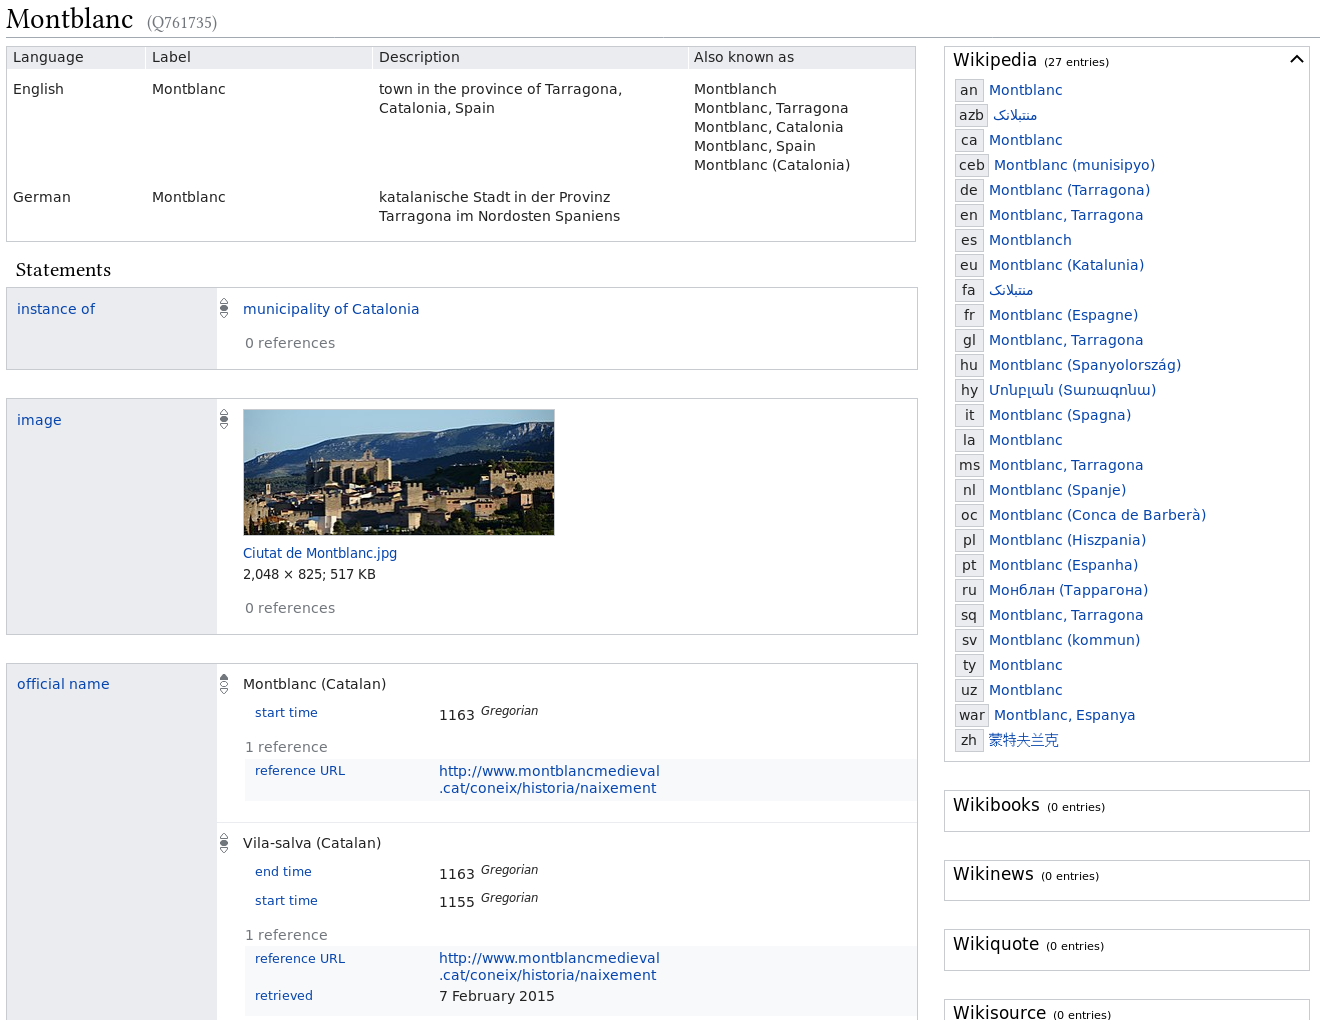
\includegraphics[width=\textwidth]{screenshots/montblanc-en}
  \end{subfigure}
\end{figure}
\begin{figure}\ContinuedFloat
  \begin{subfigure}{\textwidth}
    \caption{The \gls{item} viewed as an anonymous user, explicitly requested in the Catalan language.}
    \label{fig:montblanc-ca}
    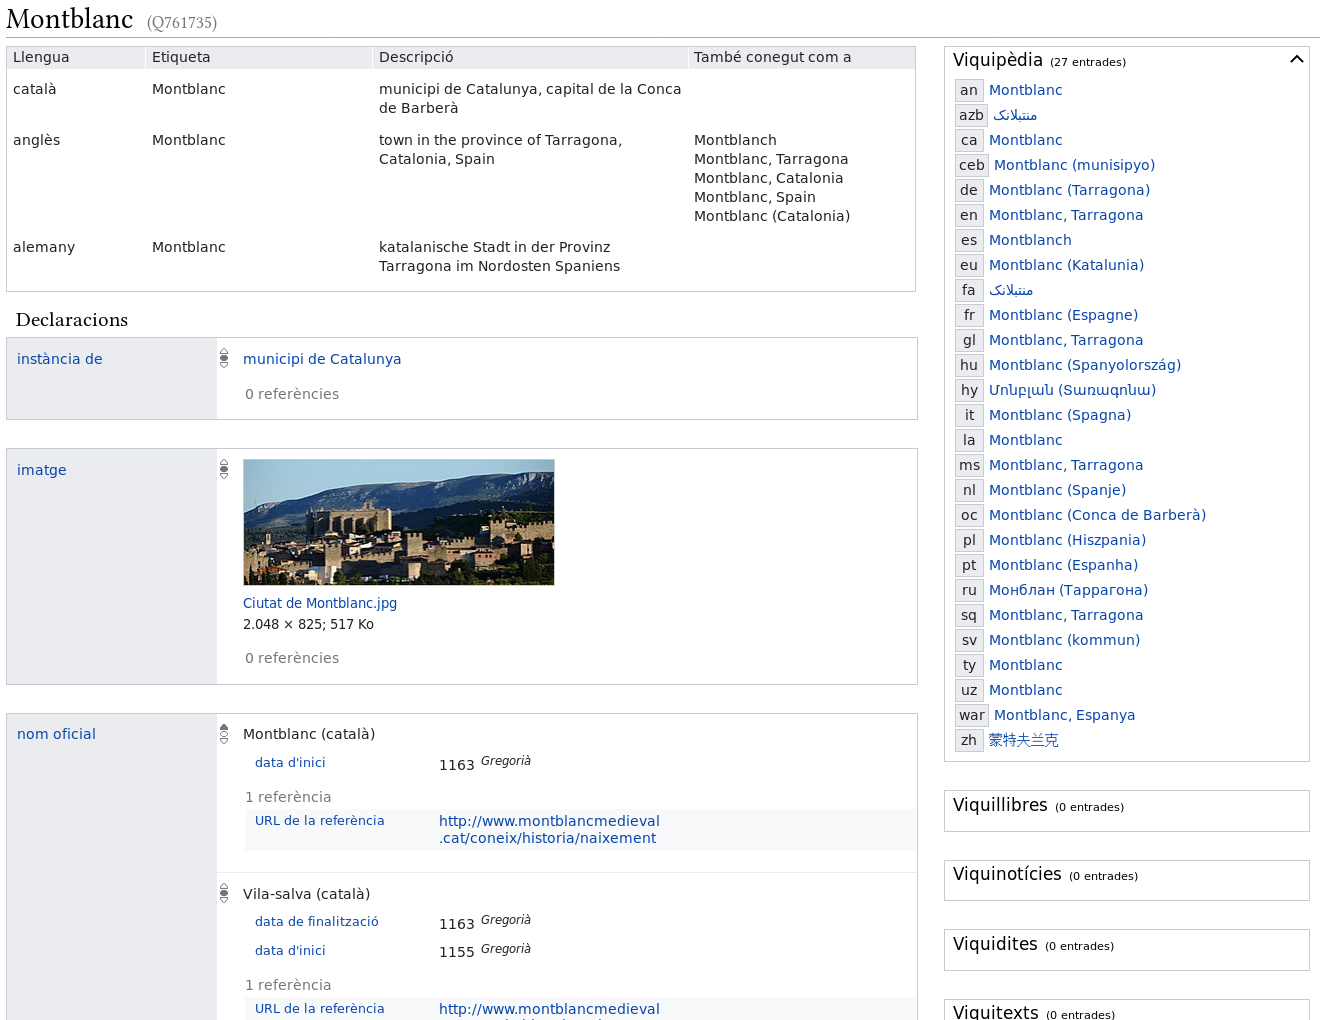
\includegraphics[width=\textwidth]{screenshots/montblanc-ca}
  \end{subfigure}
\end{figure}

It is vital to observe that there is no kind of \gls{schema} inherent to the \gls{Wikidata} data model.
Any \gls{property} can be used on any \gls{item}:
nothing in the software stops one from adding, say,
a “date of birth” \gls{statement} to an \gls{item} for a lake,
or a “parent taxon” \gls{statement} to an \gls{item} for a movie teaser poster.
The community has several ways to describe \glspl{schema} to varying degrees of formality
(such as \gls{property} lists on WikiProject pages or the property constraints system),
but they are all realized by community consensus,
not enforced by the \gls{Wikidata} software.
The great flexibility which this lends to the community
is considered to be one of \gls{Wikidata}’s greatest strengths \cite{vrandecic-restricting-the-world},
and though the use of \gls{shex}
on \gls{Wikidata} will provide another,
highly formal way to describe \glspl{schema},
there is no intention to change this fundamental operating principle of \gls{Wikidata}.

\Gls{Wikidata}’s data model, as described above,
is not directly related to \gls{rdf}.
However, to enable usage of \gls{rdf} technologies and interoperation with \gls{rdf}-based data sets,
\gls{Wikidata}’s data is exported to \gls{rdf}:
the data about any \gls{item} can be downloaded in various \gls{rdf} formats through a \gls{Linked Data} interface,
and a full, up-to-date \gls{rdf} export of \gls{Wikidata} is available in \gls{wdqs},
a \gls{sparql} endpoint to which anyone may submit queries.
In the \gls{Wikidata} \gls{rdf} exports,
items use the \gls{prefix} \prefix{wd:} and properties in a statement use the \gls{prefix} \prefix{wdt:}.
For example, the statement
\begin{quotation}
  \QL{Q7251}{Alan Turing}’s \PL{P19}{place of birth} was \QL{Q122744}{Maida Vale}
\end{quotation}
is represented in \gls{rdf} as the \gls{triple} \lstinline[language=sparql]{wd:Q7251 wdt:P19 wd:P12274}.
% TODO review layout of this statement/quote. (Using it inline is problematic because of ““double quotes””.)

% TODO explain some fundamental properties? P31, P279?

\section{Shape Expressions}
\label{sec:Background:ShEx}

% TODO somewhere, there needs to be a clear explanation why it’s so okay for us to constantly discard type links. here? not sure
% TODO example for validation

\acrfull{shex} \cite{shex}
is a standard for describing data shapes within an \gls{rdf} graph,
developed by the \gls{shex} Community Group under the umbrella of the \gls{w3c}.
A \gls{shex} \gls{schema} consists of a number of \glspl{shape},
each of which describes the layout of an \gls{rdf} \gls{resource},
called the \gls{focus node}.
The notation for \gls{shex} \glspl{schema} used in this thesis is \gls{shexc},
and while a full introduction to \gls{shex} and \gls{shexc} is beyond the scope of this thesis,
the relevant elements are described below.
For a more complete and detailed introduction,
see the \gls{shex} Primer \cite{shex-primer}.

In \gls{shexc}, a \gls{shape} definition begins with the \gls{shape}’s name (an \gls{iri})
and is followed by a block of \glspl{triple constraint} enclosed in curly braces (\lstinline!{}!).
The \glspl{triple constraint} are separated by semicolons (\lstinline{;})
and place restrictions on \glspl{triple} with the \gls{focus node} as the \gls{subject} and a certain \gls{predicate}:
a \gls{triple constraint} consists of the \gls{iri} for the \gls{predicate} and then a constraint on the \gls{object} (the value).
The value constraint can require the value to be a literal with a certain datatype,
expressed directly via the datatype’s \gls{iri},
or it can require the value to be a \gls{resource} matching another \gls{shape},
indicated by that \gls{shape}’s name (an \gls{iri}) following an \lstinline{@} symbol.
The value constraint may be followed by a cardinality for the \gls{triple constraint}:
instead of the default cardinality “must occur exactly once”,
the symbol \lstinline{?} may be appended to signify “zero or one times”
(an optional \gls{triple constraint}),
\lstinline{*} means “zero or more”
(any number of \glspl{triple} with this \gls{predicate} may occur,
but if they do occur, their \glspl{object} must still match the \gls{value constraint}),
and \lstinline{+} means “one or more”.
Multiple possible \glspl{triple constraint} for the same \gls{predicate} can be expressed
by grouping them inside parentheses (\lstinline{()}), separated by vertical bars (\lstinline{|}).

\begin{lstfloat}
\begin{lstlisting}[language=sparql]
ex:CreativeWork {
  ex:title rdf:langString;
  (
    ex:author @ex:Person+ |
    ex:author @ex:Organization
  );
  ex:cites @ex:CreativeWork*;
  ex:publicationDate xsd:dateTime?
}

ex:Person {
  ex:name rdf:langString;
  ex:dateOfBirth xsd:dateTime?
}

ex:Organization {
  ex:name rdf:langString+
}
\end{lstlisting}
\caption{An example \gls{schema} for creative works and their authors.}
\label{listing:shex-example}
\end{lstfloat}

For example, the schema in \cref{listing:shex-example} defines three \glspl{shape}
for creative works and their authors.
It describes a creative work as having a title, a string in a certain language;
being written by one or more persons or an organization;
citing any number of other creative works;
and optionally having been published on a certain date and time.
(Scholarly articles would typically have human authors,
cite multiple works and have a publication date,
whereas a documentation page could be attributed to an organization as a whole
and have no significant citations or publication date.)
A person in this \gls{schema} has exactly one name in one language
(which is not generally true \cite{falsehoods-programmers-believe-about-names},
but violations of this should be rare enough
that they are worth investigating as potential errors)
and may have a date of birth, if known.
An organization does not have any properties other than at least one name
(it may have several, e.~g. in different languages or jurisdictions).

% TODO also add example of validation with results?

By default, \gls{shex} \glspl{shape} are not \emph{closed}:
the graph may contain additional \glspl{triple} with the \gls{focus node} as the \gls{subject}
whose \glspl{predicate} do not match any of the \glspl{triple constraint} in the \gls{shape}.
For example, an organization with an \PName{ex:dateOfIncorporation} would still match the \PName{ex:Organization} shape in \cref{listing:shex-example}
even though that \gls{schema} does not mention an \PName{ex:dateOfIncorporation} \gls{predicate} anywhere.
This means that removing all \glspl{triple constraint} with a certain \gls{predicate} from a \gls{shape}
will never cause a previously matching \gls{focus node} to no longer match the \gls{shape}.
% TODO I feel like this is missing one or two sentences at the end

\section{\gls{RDF2Graph}}
\label{sec:Background:RDF2Graph}

\Gls{RDF2Graph} \cite{vanDam2015}
is a tool to automatically determine the structure of an \gls{rdf} graph
and export it as a \gls{shex} \gls{schema}
(other output formats are also supported).
It relies heavily on the type information of each node and the class hierarchy in the graph,
determining the valid \glspl{predicate} and their value types and cardinalities for each type in the graph.
There is also an optional step to simplify the resulting \gls{schema}.

To discover the structure of an \gls{rdf} graph,
\gls{RDF2Graph} runs a set of queries against a \gls{sparql} endpoint serving that graph.
(This can be a local server, perhaps simply based on a single file containing the graph,
or a remote server.)
It enumerates all the classes that occur in the graph
and then collects all the \glspl{predicate} that are used on instances of each class.
For each \gls{predicate} of each class,
it then gets the types referenced in the values for those \glspl{predicate}
(usually the classes of the referenced nodes,
but values can also be literals or external references),
as well as forward and reverse multiplicity for each such type link.
All this information is stored in a separate \gls{rdf} graph private to \gls{RDF2Graph}.

If the simplification step is enabled,
\gls{RDF2Graph} will afterwards apply some transformations to the structure
based on the hierarchy of the classes involved,
which happens in several steps.
The following description uses the same step numbers as \cite{vanDam2015},
but elides several steps which are mostly implementation details,
which is why the step numbers are not consecutive here.
See \cite{vanDam2015} and the \gls{RDF2Graph} source code for the full description.
(In the source code, the steps are counted as sub-steps of the general step 7.4 “simplification”:
for example, step 2 is implemented under a code comment for “7.4.2”.)

% TODO review the layout of the listings here
% TODO some of the listings are too high for their page. perhaps remove blank lines between shapes

In step 2, all \glspl{predicate} from child classes are copied to parent classes.
For example, in \cref{fig:simplify-7.4.2},
the \PName{ex:WebResource} and \PName{ex:CreativeWork} classes are initially empty
but then inherit several \glspl{predicate} from their child classes.
(The \lstinline{.} in the \PName{ex:url} \gls{value constraint} means “any value”.)

\begin{lstfloat}[ht]
\begin{sublstfloat}[t]{0.45\textwidth}
\begin{lstlisting}[showlines=true]
ex:CreativeWork {}

ex:ScholarlyArticle
    EXTENDS ex:CreativeWork {
  ex:title rdf:langString;
  ex:author @ex:Person+;
  ex:cites @ex:CreativeWork+;
}

ex:WebResource
    EXTENDS ex:CreativeWork {}

ex:BlogPost
    EXTENDS ex:WebResource {
  ex:url .;
  ex:title rdf:langString;
  (
    ex:author @ex:Person |
    ex:author @ex:Organization
  );
}

ex:DocumentationPage
    EXTENDS ex:BlogPost {
  ex:url .;
  ex:title rdf:langString;
  ex:author @ex:Organization;
}















\end{lstlisting}
\caption{Before step 2.}
\label{fig:simplify-7.4.2-before}
\end{sublstfloat}
\begin{sublstfloat}[t]{0.45\textwidth}
\begin{lstlisting}
ex:CreativeWork {
  ex:url .;
  ex:title rdf:langString;
  (
    ex:author @ex:Person+ |
    ex:author @ex:Organization
  );
  ex:cites @ex:CreativeWork+;
}

ex:ScholarlyArticle
    EXTENDS ex:CreativeWork {
  ex:title rdf:langString;
  ex:author @ex:Person+;
  ex:cites @ex:CreativeWork+;
}

ex:WebResource
    EXTENDS ex:CreativeWork {
  ex:url .;
  ex:title rdf:langString;
  (
    ex:author @ex:Person |
    ex:author @ex:Organization
  );
}

ex:BlogPost
    EXTENDS ex:WebResource {
  ex:url .;
  ex:title rdf:langString;
  (
    ex:author @ex:Person |
    ex:author @ex:Organization
  );
}

ex:DocumentationPage
    EXTENDS ex:WebResource {
  ex:url .;
  ex:title rdf:langString;
  ex:author @ex:Organization;
}
\end{lstlisting}
\caption{After step 2.}
\label{fig:simplify-7.4.2-after}
\end{sublstfloat}
\caption[Simplification step 2.]{Simplification step 2 (in \gls{shexc}-like pseudo-syntax).}
\label{fig:simplify-7.4.2}
\end{lstfloat}

Step 3 removes \glspl{predicate} which are only found in a single subclass
from the parent class again.
In the example from \cref{fig:simplify-7.4.2},
the \PName{ex:cites}  and \PName{ex:url} \glspl{predicate} will be removed from the \PName{ex:CreativeWork} \gls{shape}
because they are only found in one subclass
(\PName{ex:ScholarlyArticle} and \PName{ex:WebResource}, respectively),
while the other \glspl{predicate} will be kept.
In the \PName{ex:WebResource} \gls{shape} itself,
all \glspl{predicate} will be kept because they occur in both subclasses,
\PName{ex:BlogPost} and \PName{ex:DocumentationPage}.
See \cref{fig:simplify-7.4.3} for the result.

\begin{lstfloat}[ht]
\begin{sublstfloat}[t]{0.45\textwidth}
\begin{lstlisting}
ex:CreativeWork {
  ex:url .;
  ex:title rdf:langString;
  (
    ex:author @ex:Person+ |
    ex:author @ex:Organization
  );
  ex:cites @ex:CreativeWork+;
}

ex:ScholarlyArticle
    EXTENDS ex:CreativeWork {
  ex:title rdf:langString;
  ex:author @ex:Person+;
  ex:cites @ex:CreativeWork+;
}

ex:WebResource
    EXTENDS ex:CreativeWork {
  ex:url .;
  ex:title rdf:langString;
  (
    ex:author @ex:Person |
    ex:author @ex:Organization
  );
}

ex:BlogPost
    EXTENDS ex:WebResource {
  ex:url .;
  ex:title rdf:langString;
  (
    ex:author @ex:Person |
    ex:author @ex:Organization
  );
}

ex:DocumentationPage
    EXTENDS ex:WebResource {
  ex:url .;
  ex:title rdf:langString;
  ex:author @ex:Organization;
}
\end{lstlisting}
\caption{Before step 3.}
\label{fig:simplify-7.4.3-before}
\end{sublstfloat}
\begin{sublstfloat}[t]{0.45\textwidth}
\begin{lstlisting}[showlines=true]
ex:CreativeWork {
  ex:title rdf:langString;
  (
    ex:author @ex:Person+ |
    ex:author @ex:Organization
  );
}

ex:ScholarlyArticle
    EXTENDS ex:CreativeWork {
  ex:title rdf:langString;
  ex:author @ex:Person+;
  ex:cites @ex:CreativeWork+;
}

ex:WebResource
    EXTENDS ex:CreativeWork {
  ex:url .;
  ex:title rdf:langString;
  (
    ex:author @ex:Person |
    ex:author @ex:Organization
  );
}

ex:BlogPost
    EXTENDS ex:WebResource {
  ex:url .;
  ex:title rdf:langString;
  (
    ex:author @ex:Person |
    ex:author @ex:Organization
  );
}

ex:DocumentationPage
    EXTENDS ex:WebResource {
  ex:url .;
  ex:title rdf:langString;
  ex:author @ex:Organization;
}


\end{lstlisting}
\caption{After step 3.}
\label{fig:simplify-7.4.3-after}
\end{sublstfloat}
\caption[Simplification step 3.]{Simplification step 3 (in \gls{shexc}-like pseudo-syntax).}
\label{fig:simplify-7.4.3}
\end{lstfloat}

After that, in step 4 all references which are still found in a parent class
are removed from the child classes, where they are now redundant.
In \cref{fig:simplify-7.4.4}, this mostly clears the \gls{schema}:
most \glspl{predicate} are found in \PName{ex:CreativeWork},
and only \PName{ex:WebResource} retains another \gls{predicate}, \PName{ex:url}.
Note that this step was later disabled, see \cref{sec:RDF2Graph+Wikidata:updates}.

\begin{lstfloat}[ht]
\begin{sublstfloat}[t]{0.45\textwidth}
\begin{lstlisting}
ex:CreativeWork {
  ex:title rdf:langString;
  (
    ex:author @ex:Person+ |
    ex:author @ex:Organization
  );
}

ex:ScholarlyArticle
    EXTENDS ex:CreativeWork {
  ex:title rdf:langString;
  ex:author @ex:Person+;
  ex:cites @ex:CreativeWork+;
}

ex:WebResource
    EXTENDS ex:CreativeWork {
  ex:url .;
  ex:title rdf:langString;
  (
    ex:author @ex:Person |
    ex:author @ex:Organization
  );
}

ex:BlogPost
    EXTENDS ex:WebResource {
  ex:url .;
  ex:title rdf:langString;
  (
    ex:author @ex:Person |
    ex:author @ex:Organization
  );
}

ex:DocumentationPage
    EXTENDS ex:WebResource {
  ex:url .;
  ex:title rdf:langString;
  ex:author @ex:Organization;
}
\end{lstlisting}
\caption{Before step 4.}
\label{fig:simplify-7.4.4-before}
\end{sublstfloat}
\begin{sublstfloat}[t]{0.45\textwidth}
\begin{lstlisting}[showlines=true]
ex:CreativeWork {
  ex:title rdf:langString;
  (
    ex:author @ex:Person+ |
    ex:author @ex:Organization
  );
}

ex:ScholarlyArticle
    EXTENDS ex:CreativeWork {}

ex:WebResource
    EXTENDS ex:CreativeWork {
  ex:url .;
}

ex:BlogPost
    EXTENDS ex:WebResource {}

ex:DocumentationPage
    EXTENDS ex:WebResource {}




















\end{lstlisting}
\caption{After step 4.}
\label{fig:simplify-7.4.4-after}
\end{sublstfloat}
\caption[Simplification step 4.]{Simplification step 4 (in \gls{shexc}-like pseudo-syntax).}
\label{fig:simplify-7.4.4}
\end{lstfloat}

Step 2 also merges references to parent classes,
and the other steps take this into account by respecting subclass relations as well.
For example, consider the initial \gls{schema} in \cref{fig:simplify-classes}.
Initially, it states that scholarly articles only cite other scholarly articles,
and web resources only cite other web resources;
after simplification, it states that creative works cite other creative works of any kind:
the references to \PName{ex:ScholarlyArticle} and \PName{ex:WebResource}
were merged while copying the \PName{ex:cites} predicate into the \PName{ex:CreativeWork} parent class,
and afterwards the individual \glspl{predicate} were removed from the child classes
because they are covered by the merged reference in the parent class.

\begin{lstfloat}[ht]
\begin{sublstfloat}[t]{0.45\textwidth}
\begin{lstlisting}
ex:CreativeWork {}

ex:ScholarlyArticle
    EXTENDS ex:CreativeWork {
  ex:cites @ex:ScholarlyArticle+
}

ex:WebResource
    EXTENDS ex:CreativeWork {
  ex:cites @ex:WebResource*
}
\end{lstlisting}
\caption{Before simplification.}
\label{fig:simplify-classes-before}
\end{sublstfloat}
\begin{sublstfloat}[t]{0.45\textwidth}
\begin{lstlisting}[showlines=true]
ex:CreativeWork {
  ex:cites @ex:CreativeWork*
}

ex:ScholarlyArticle
    EXTENDS ex:CreativeWork {}

ex:WebResource
    EXTENDS ex:CreativeWork {}


\end{lstlisting}
\caption{After simplification.}
\label{fig:simplify-classes-after}
\end{sublstfloat}
\caption[Simplification, with class relations.]{
  Simplification (in \gls{shexc}-like pseudo-syntax), with class relations.
  (This example is independent from the previous example.)
}
\label{fig:simplify-classes}
\end{lstfloat}

At this point, the information which \gls{RDF2Graph} extracted is available in a private \gls{rdf} graph.
From there, it can be exported into various formats by different exporters.
The \gls{shex} exporter loads parts of these results into a temporary \gls{rdf} database of its own,
applies some transformations to them via \gls{sparql},
converts them to \gls{json-ld},
further transforms the \gls{json},
and finally exports the result into \gls{shexc} text via the Jade template engine.

\section{Wikimedia Toolforge}
\label{sec:Background:Toolforge}

Wikimedia Toolforge is a hosting environment provided by the Wikimedia Foundation
where trusted members of the \gls{Wikimedia} community may host and develop their “tools” or other work.
Most tools are web-based and reachable under the \href{https://tools.wmflabs.org/}{tools.wmflabs.org} domain,
but it is also possible to run bots or analysis jobs on Toolforge.
Tools can be written in a variety of languages
(e.~g. PHP, Python, Java, \gls{JavaScript})
and have access to live replicas of the \gls{Wikimedia} production databases,
data dumps of \gls{Wikimedia} projects,
custom tool-specific databases,
and a Sun Grid Engine job execution system for long-running or resource-intensive tasks.

%% LaTeX2e class for student theses
%% sections/content.tex
%% 
%% Karlsruhe Institute of Technology
%% Institute for Program Structures and Data Organization
%% Chair for Software Design and Quality (SDQ)
%%
%% Dr.-Ing. Erik Burger
%% burger@kit.edu
%%
%% Version 1.3.3, 2018-04-17

\chapter{Applying \gls{RDF2Graph} to Wikidata}
\label{ch:RDF2Graph+Wikidata}

This chapter describes the changes that were made to \gls{RDF2Graph} and related software in the course of this thesis.
Some of them are general improvements unrelated to \gls{Wikidata} (\cref{sec:RDF2Graph+Wikidata:updates}),
some are motivated by the \gls{Wikidata} use case but still generally useful (\cref{sec:RDF2Graph+Wikidata:cyclic-graphs,sec:RDF2Graph+Wikidata:schema-reduction,sec:RDF2Graph+Wikidata:depth-limit}),
and some are specific to \gls{Wikidata} and result in a version of \gls{RDF2Graph}
that cannot be used for other RDF graphs (\cref{sec:RDF2Graph+Wikidata:Wikidata}).
All the changes are available in the source code repositories at
\url{https://github.com/lucaswerkmeister/RDF2Graph} and
\url{https://github.com/lucaswerkmeister/RDFSimpleCon},
in the \branchname{master} and \branchname{wikidata} branches;
some of them may also be merged into the upstream \gls{RDF2Graph} and \gls{RDFSimpleCon} repositories in the future.

\section{General \gls{RDF2Graph} Updates}
\label{sec:RDF2Graph+Wikidata:updates}

The \branchname{master} branch of the \gls{RDF2Graph} source code repository
has not seen any updates since 2015 (when \cite{vanDam2015} was published),
so some updates were needed to make the program run on newer software versions
and to target a more recent version of \gls{shex}.
Many of these were rather minor in nature,
but a few of the major ones concerning the \gls{shex} exporter are described in this section.
(I later noticed that the \gls{RDF2Graph} source code repository
also has a \branchname{dev} branch,
which has some more recent changes including a few fixes,
but most of them are not relevant to the issues discussed here.)

The final step of the \gls{shex} export was mostly rewritten from scratch.
This is the step that translates a \gls{json-ld} file describing the \glspl{shape} of the \gls{schema}
into a \gls{shexc} file;
the previous version did this using Jade,
a templating engine for \gls{html} documents (renamed to Pug in 2016),
constructing an \gls{html} document containing a single plain-text \lstinline[language=html]{<pre>} element,
then extracting this text from the document using an \gls{html}-to-text converter.
The new version directly produces the text from \gls{JavaScript}
and includes several improvements:
datatypes are now properly supported,
whereas the previous version only supported a handful of hard-coded \glspl{iri} as datatypes
and exported all other datatypes as if they were actually \glspl{shape};
\glspl{prefix} are used everywhere in the output, highly improving readability;
and the output is sorted, making the whole generation process more deterministic
and thus making it easier to compare the results of multiple inference processes.

The syntax of the generated \gls{shexc} \glspl{schema}
also required some changes.
First, \gls{RDF2Graph} originally targeted \gls{shex} version 1.0
whereas the current release is version 2.0,
which introduced some syntactic changes
(e.~g. replacing some commas with semicolons).
Second, \gls{RDF2Graph} emitted syntax for an experimental, in-progress version of \gls{shex}
with support for inheritance between \glspl{shape}:
if, for example, the inferred \gls{schema} contained classes for both “human” and “person”,
and “human” was a subclass of “person” in the input data set,
then \gls{RDF2Graph} would declare that the “human” \gls{shape} extended the “person” \gls{shape}
and omit \glspl{predicate} from the “person” \gls{shape} in the “human” \gls{shape},
since those would be redundant with the \glspl{predicate} inherited from the “person” \gls{shape}.
This feature has not made it into any released version of \gls{shex} yet
(it can still be found in \branchname{on-shape-expression} branches of related repositories,
though the syntax has slightly changed:
it now uses the keyword \lstinline{EXTENDS} whereas \gls{RDF2Graph} used the symbol \lstinline{&}),
so the \gls{shex} exporter was changed to only mention the parent classes for a \gls{shape} in a comment,
and simplification step 4 (see \cref{sec:Background:RDF2Graph}) was disabled
so that the redundant \glspl{predicate} are included after all,
since they are no longer automatically inherited.

\section{Wikidata Support}
\label{sec:RDF2Graph+Wikidata:Wikidata}

This section outlines the general process that is used when running \gls{RDF2Graph} against data from \gls{Wikidata}
and then describes several changes to \gls{RDF2Graph} that were necessary to support this.
(The subsequent subsections correspond to those changes, not to the individual steps of the process.)

\subsection{Overall process, data download}
\label{subsec:RDF2Graph+Wikidata:Wikidata:download}

Usually, \gls{RDF2Graph} is run against a \gls{sparql} endpoint
which serves the \gls{rdf} graph for which one wants to infer the structure.
However, simply running \gls{RDF2Graph} against \acrfull{wdqs}, the public \gls{sparql} endpoint for \gls{Wikidata},
would mean attempting to infer a \gls{schema} from all of \gls{Wikidata},
which is neither the goal of this thesis
(that is to infer \glspl{schema} from a small set of exemplary \glspl{item})
nor even remotely feasible given the amount of data in \gls{Wikidata}
(for example, the 2018-08-20 full \gls{Wikidata} dump, uncompressed,
is \SI{309.7}{\giga\byte} large and \num{8316156305} lines long).

Instead, a process was set up which,
given a query which selects the exemplary \glspl{item},
downloads the related data for them and runs \gls{RDF2Graph} against it.
The process is outlined in \cref{fig:process}
and controlled by a Makefile in the \gls{RDF2Graph} repository,
so that after creating an \filename{\variable{example}.entities.sparql} file
with a \gls{sparql} query selecting the exemplary items,
it is sufficient to run \command{make \variable{example}.shex}
to run the entire process and generate the \gls{shex} file.

\begin{figure}
  \centering
  \begin{tikzpicture}
    \tikzstyle{file} = [rectangle, draw, rounded corners, text centered]
    \tikzstyle{pipe} = [style=file, dashed]
    \tikzstyle{directory} = [rectangle, draw, text centered]
    \tikzstyle{arrow} = [draw, -latex', right]

    \begin{scope}[node distance=2cm]
      \node[file] (entities) {\filename{\variable{example}.entities.sparql}};
      \node[file, below of=entities] (data) {\filename{\variable{example}.data.sparql}};
      \node[pipe, below of=data] (JSON) {\filename{\variable{example}.json}};
      \node[file, below of=JSON] (N-Triples) {\filename{\variable{example}.nt}};
      \node[directory, below of=N-Triples] (Fuseki) [align=center] {\dirname{\variable{example}-fuseki} \\ \texttt{http://localhost:3030/\variable{example}/query}};
      \node[directory, below of=Fuseki] (RDF2Graph) {\dirname{\variable{example}-results}};
      \node[file, below of=RDF2Graph] (ShEx) {\filename{\variable{example}.shex}};
      \node[file, below of=ShEx] (HTML) {\filename{\variable{example}.html}};
    \end{scope}

    \begin{scope}[every path/.style=arrow, midway]
      \path (entities) -- node {\command{sed}} (data);
      \path (data) -- node {\gls{wdqs}} (JSON);
      \path (JSON) -- node {\command{jq}} (N-Triples);
      \path (N-Triples) -- node {Fuseki} (Fuseki);
      \path (Fuseki) -- node {\gls{RDF2Graph}} (RDF2Graph);
      \path [dashed] (RDF2Graph.north east) to [out=30,in=330,looseness=5] node {\gls{RDF2Graph}, simplify} (RDF2Graph.south east);
      \path (RDF2Graph) -- node {\gls{shex} exporter} (ShEx);
      \path (ShEx) -- node {\command{pygmentize}} (HTML);
    \end{scope}
  \end{tikzpicture}
  \caption{Overview of the process}
  \label{fig:process}
\end{figure}

First, the query selecting the exemplary \glspl{item} is transformed
into a query selecting all the required data,
using the Unix \command{sed} command.
The generated query selects all \glspl{statement} of the exemplary \glspl{item} (“direct \glspl{statement}”),
all \glspl{statement} of \glspl{item} which occur as values of the direct \glspl{statement} (“indirect \glspl{statement}”),
and all \PL{P31}{instance of} \glspl{statement} of \glspl{item} which occur as values of the indirect \glspl{statement}.
This query is run against \gls{wdqs},
which returns the results in \gls{json} format;
they are then piped into a script for the \command{jq} tool (“\gls{json} query”),
which transforms them into \gls{N-Triples} format,
and stored in an \gls{N-Triples} file.

Next, the Apache Jena Fuseki \gls{sparql} server is run locally,
serving the data from this \gls{N-Triples} file.
As soon as it has finished loading the data file,
\gls{RDF2Graph} is run against this local \gls{sparql} endpoint for the main inference process,
including \gls{RDF2Graph}’s simplification step.
Once \gls{RDF2Graph} terminates, the Fuseki server is stopped.

Afterwards, the results from \gls{RDF2Graph} are available as a graph of classes with associated information,
and the \gls{RDF2Graph} \gls{shex} exporter is run to produce a \gls{shex} file.
If desired (\command{make \variable{example}.html}),
that file can also be turned into an \gls{html} file using the Pygments syntax highlighter,
which makes the \gls{shex} code more readable.

% TODO look over the subsections again.
% in general, each should first introduce a problem and then state my solution.
% some of them should also probably be longer than one paragraph

\subsection{Type predicates}
\label{subsec:RDF2Graph+Wikidata:Wikidata:predicates}

The most fundamental change to make \gls{RDF2Graph} support \gls{Wikidata}
was % TODO is?
to change the type predicates used.
\Gls{RDF2Graph} heavily relies on the type information of the RDF graph it inspects,
assuming a one-to-one mapping between classes and \glspl{shape},
and it uses the standard \glspl{predicate} \PName{rdf:type} and \PName{rdfs:subClassOf}
to determine the class of a subject and the superclasses of a class, respectively.
However, \gls{Wikidata} does not use these standard \glspl{predicate}:
the class(es) and superclass(es) of an item
are regular \glspl{statement} like any other \gls{Wikidata} \gls{statement},
using the \glspl{property} \PL{P31}{instance of} and \PL{P279}{subclass of}.
In the \gls{rdf} export, \PName{rdf:type} and \PName{rdfs:subClassOf} are only used
as part of the meta-model, % TODO meta-model? hm
assigning each item the class \PName{wikibase:Item}, a subclass of \PName{wikibase:Entity}.
To use the type information within the data instead of this meta-model,
\gls{RDF2Graph} was changed to use the \glspl{predicate} \PName{wdt:P31} and \PName{wdt:P279}
instead of \PName{rdf:type} and \PName{rdfs:subClassOf}.

\subsection{Data reduction}
\label{subsec:RDF2Graph+Wikidata:Wikidata:reduction}

During the data download step, some data is dropped from the \glspl{item}.
For one, the \glspl{label}, \glspl{description} and \glspl{alias} of an \gls{item} can make up a large portion of its data,
but are generally not interesting for \gls{shex} \glspl{schema},
since there is rarely more to say about them than
“an \gls{item} has one or more \glspl{label}, zero or more \glspl{description}, and zero or more \glspl{alias}”.
(A manually curated \gls{schema} might go beyond this –
perhaps requiring, for example, that \glspl{item} about Spanish municipalities have a label in Spanish –
but such details are beyond the ability of \gls{RDF2Graph} to infer.)
Additionally, \gls{Wikidata} \glspl{item} often have a number of \glspl{statement} listing external identifiers for the \gls{item}
(that is, identifiers in other databases for the same concept described by this \gls{item}):
for example, \gls{Wikidata}’s \Q{Q80} corresponds to \loc{no99010609} in the \gls{loc},
\viaf{85312226} in \gls{viaf},
\imdbName{nm3805083} in the \gls{imdb},
\TwitterAccount{timberners\_lee} on Twitter,
and dozens of other external identifiers.
All these external identifiers are technically just ordinary \glspl{statement},
but since they carry a rather different kind of information than other \glspl{statement},
they are sorted into a separate section when viewing the \gls{item} on the \gls{Wikidata} website.
To reduce the runtime of the \gls{RDF2Graph} inference process,
and to reduce clutter in the inferred \glspl{schema},
the \glspl{label}, \glspl{description}, \glspl{alias}, and external identifiers of an \gls{item}
are therefore excluded when downloading the data for a set of exemplary \glspl{item}.

\subsection{Full type hierarchy}
\label{subsec:RDF2Graph+Wikidata:Wikidata:hierarchy}

However, one unfortunate consequence of running \gls{RDF2Graph} against a reduced data set
is that \gls{RDF2Graph} cannot see the full type hierarchy of the classes involved:
for example, depending on how much data was downloaded,
it may or may not be aware that the classes \QL{Q112099}{island nation} and \QL{Q3624078}{sovereign state}
have a common superclass, \QL{Q7275}{state},
which reduces the available options during the simplification step. % TODO not happy with this phrasing
To mitigate this, \gls{RDF2Graph} was patched
to allow specifying an alternative \gls{sparql} endpoint for all queries that require a full view of the data,
and uses this alternative endpoint for the query to get all parent and child classes of a class.
The Makefile mentioned in \cref{subsec:RDF2Graph+Wikidata:Wikidata:download}
specifies the \gls{wdqs} \gls{sparql} endpoint for this option,
so that \gls{RDF2Graph} can learn the full class hierarchy around all relevant items % TODO is “learn” the right word?
even when running against a subset of \gls{Wikidata}. % TODO “subset of Wikidata”? not quite happy with that phrasing

\subsection{Simplification}
\label{subsec:RDF2Graph+Wikidata:Wikidata:simplification}

The simplification process also required some changes to support \gls{Wikidata}.
Originally, \gls{RDF2Graph} would merge all classes into their superclass,
almost completely unconditionally,
stopping only at the root class \PName{owl:Thing}.
This was much too aggressive for \gls{Wikidata}:
not only does \gls{Wikidata} have a different root class (\QL{Q35120}{entity}),
but it also has a complex hierarchy of abstract classes below that root class,
and merging other classes into those abstract classes
(like \QL{Q151885}{concept}, \QL{Q7184903}{abstract object} or \QL{Q830077}{subject})
would not result in useful \glspl{schema}.
Therefore, step 2 in the simplification process was adapted
to add a number of \gls{Wikidata} \glspl{item} to the set of classes which other classes should not be merged into
(originally only containing \PName{owl:Thing}),
and to stop looking for common superclasses of two classes after checking five levels in the class hierarchy.
(The limit of five levels is an arbitrary choice
and could also be made configurable if deemed necessary in the future.) % TODO look a bit more into this?

\section{Support for Cyclic Type Hierarchies}
\label{sec:RDF2Graph+Wikidata:cyclic-graphs}
% TODO this whole section mixes parent/child and parent class / subclass terminology :/

As outlined in \cref{sec:Background:RDF2Graph},
\gls{RDF2Graph} has an optional simplification feature
where the \gls{schema} will be simplified in several steps,
based on the type hierarchy of the classes involved.
For this, the type hierarchy is loaded into an in-memory data structure,
which in the code is referred to as a \emph{tree}. % TODO is the emphasis here appropriate? feels odd
In fact, the data structure forms a generic, directed graph,
where each node may have any number of children and any number of parents,
and no restrictions on the structure are enforced during construction.
However, while the algorithms subsequently operating on the data structure support classes with multiple parent classes,
they do assume that the graph is acyclic,
i.~e., that no class is an indirect subclass of itself.

This assumption makes sense in general,
since a type hierarchy is usually assumed to be acyclic:
if there is a cycle in the subclass relations between a list of classes,
that effectively renders all these classes equivalent,
since any instance of any one of these classes is then also an (indirect) instance of all other classes.
However, experience shows % TODO “experience shows” sounds extremely dodgy
that occasional emergence of subclass cycles is almost unavoidable on \gls{Wikidata}:
any one of the subclass links may appear reasonable for just the two \glspl{item} it connects,
and an editor looking at these \glspl{item} will not necessarily notice that a cycle has been formed,
since the other statements forming the cycle are not visible when looking at these two \glspl{item}.
For example, as of 2018-10-11, % TODO date macro?
there exists a cycle in \gls{Wikidata} in the following classes:
\QL{Q4393498}{representation}, \QL{Q937228}{property}, \QL{Q714737}{category of being},
\QL{Q151885}{concept}, \QL{Q2145290}{mental representation}, \QL{Q4393498}{representation}.
It was first introduced in \wikidataDiff{726473098},
when the parent class of \QL{Q2145290}{mental representation}
was changed from \QL{Q1272626}{representation} to \QL{Q4393498}{representation},
and reinforced in \wikidataDiff{726473565};
the latter revision was later reverted in \wikidataDiff{735108434},
citing the created subclass loop as part of the reason,
but as the first revision was not reverted nor the \gls{item} otherwise edited since then,
the cycle persists so far.
The fact that editors work in different languages,
and different items may share the same label in the same language
(see \Q{Q1272626} and \Q{Q4393498}, both “representation”, above),
contributes to the problem that such cycles can be introduced accidentally
and the correct way to break them is not always obvious.

While these cycles are usually eventually found and fixed by the community, % TODO “usually eventually” sounds stupid
it is possible that, in the meantime, \gls{RDF2Graph} will run on a subclass graph containing cycles.
Therefore, to make the process more robust,
several algorithms in the simplification step were adjusted to be able to cope with cyclic graphs.
This is valuable even though the results in the cycle may no longer make sense,
since it means that a cycle somewhere in the class hierarchy,
typically among very abstract classes,
will no longer impede simplification in other, more concrete classes,
where simplification is much more useful anyways.

\subsection{\FunctionName{GetAllChildren}}
\label{subsec:RDF2Graph+Wikidata:cyclic-graphs:GetAllChildren}

A general component of the new algorithms are methods to get all children and parents of a node,
in a matter that is guaranteed to terminate even if there are cycles among the children or parents.
The method for collecting all child nodes is outlined in \cref{alg:GetAllChildren},
and the method for collecting all parent nodes is completely analogous.
Since each node can only enter the return set once,
the queue only grows when nodes are added to the return set,
and each iteration takes one node from the queue,
the algorithm must eventually exhaust the queue and terminate,
provided that the set of nodes reachable from the initial node is finite.
% TODO should this be a more formal proof?

% TODO it feels highly unlikely that this algorithm doesn’t have some existing name
\begin{algorithm}
  \begin{algorithmic}
    \Function{GetAllChildren}{node}
    \State $\Instruction{initialize \Variable{set} of all children (empty)}$
    \State $\Instruction{initialize working \Variable{queue} of children (empty)}$
    \State $\Instruction{add to \Variable{queue}} \gets \Instruction{direct children of \Variable{node}}$
    \While{$\Variable{queue} \neq \emptyset$}
    \State $\Variable{child} \gets \Instruction{take from \Variable{queue}}$
    \If{$\Variable{child} \not\in \Variable{set}$}
    \State $\Instruction{add to \Variable{set}} \gets \Variable{child}$
    \State $\Instruction{add to \Variable{queue}} \gets \Instruction{direct children of \Variable{child}}$
    \EndIf
    \EndWhile
    \State \Return $\Instruction{\Variable{set}}$
    \EndFunction
  \end{algorithmic}
  \caption{Algorithm to collect all direct and indirect child nodes in a graph}
  \label{alg:GetAllChildren}
\end{algorithm}

\subsection{Counting instances}
\label{subsec:RDF2Graph+Wikidata:cyclic-graphs:count-instances}

With this in place,
it becomes easy to reimplement the method which counts the number of direct and indirect instances of each class,
based on the direct instance counts on each class node.
Previously, the method operated recursively,
aggregating instance counts for each indirect subclass of a class
all the way up to the class itself,
and this recursion would never terminate when encountering a cycle of subclasses.
Instead, the new implementation collects all direct and indirect subclasses up-front using \cref{alg:GetAllChildren}
and then sums up their direct instance counts.

\subsection{Simplification steps 3 and 4}
\label{subsec:RDF2Graph+Wikidata:cyclic-graphs:simplify-step-3+4}

Two steps of the simplification process
remove some of the temporary (added) type links of a node,
based on the temporary type links of its neighboring node:
step 3 removes temporary type links from parent classes that are only found in one child class,
and step 4 removes temporary type links from child classes that are made redundant by a type link in the parent class.
Both steps were originally implemented as inspecting the neighboring nodes’ temporary type links
and then directly manipulating the node’s own temporary type links.
This required that each step traversed the nodes in the correct order
(parents before children for step 3,
children before parents for step 4)
and was implemented by traversing the graph recursively,
which is problematic if the graph contains cycles.
% TODO all this anonymous steps and parts business sounds clumsy
% give all of them numbers and/or names and then rephrase this
This problem was solved by splitting up the analysis and modification of the temporary type links:
each step now has two parts,
where the first part marks all temporary type links that should be removed,
and the second part actually removes them from a node’s temporary type links.
As long as the first part for all nodes is run before the second part for any node,
these parts can now be run in any order,
and instead of recursively traversing the graph,
both steps now first collect all child nodes of the root node
and then iterate them twice,
running the first part the first time and the second part the second time.
% TODO pseudocode algorithms for any of this paragraph?

\subsection{Node distances}
\label{subsec:RDF2Graph+Wikidata:cyclic-graph:distance}

\Gls{RDF2Graph} also has a method to determine the distance of all indirect parents from a certain node,
which is used when searching for common superclasses of a class.
Like the other methods, this was implemented recursively,
setting the distance of a parent node to the current value of a counter
and then calling the same method on all parent nodes of that node with the counter incremented by one.
In this case, the recursion was kept,
but the method was adjusted to only visit a parent node
if it has not been visited before, or if its current distance is larger than the counter value.
The second part of the condition is necessary to ensure that the distance is set correctly
if a node is visited first via a longer path and then later again via a shorter path,
which is possible since the method implements a depth-first search instead of a breadth-first search.
% TODO pseudocode for this?

\subsection{Parent check}
\label{subsec:RDF2Graph+Wikidata:cyclic-graph:IsParent}

% TODO perhaps just drop this paragraph? it’s really trivial
And finally, there is also a method to determine whether a certain node is a (direct or indirect) parent node of another node.
This was originally implemented recursively,
% TODO phrasing here feels convoluted
but could be replaced with a simple check whether the potential parent node is an element of the set of the child node’s parent nodes,
using \cref{alg:GetAllChildren}.

\section{Schema Reduction}
\label{sec:RDF2Graph+Wikidata:schema-reduction}

An unexpected problem emerged once the \gls{schema} inference itself was in place: % TODO phrasing: “in place”?
it proved to be almost impossible to validate \glspl{item} against the inferred \glspl{schema}
for all but the most simple data sets.
Two \gls{shex} implementations were evaluated:
shex.js, % TODO link? cite?
a \gls{JavaScript} implementation running in \gls{Node.js},
and shex-java,
a Java implementation offering two different validation algorithms \cite{boneva:hal-01590350}.
shex.js would usually crash with an out-of-memory error from \gls{Node.js} within a few minutes,
whereas shex-java would run for hours on end without any output or apparent progress
(with either algorithm).

One attempted strategy to be able to validate the inferred \glspl{schema} % TODO “attempted strategy”? feels awkward
was to reduce the size of the \glspl{schema} by dropping some less-relevant elements.
This was part of the motivation for dropping \glspl{label}, \glspl{description}, \glspl{alias}, and external identifiers of an \gls{item}
from the data set that the inference would be run against
(see \cref{subsec:RDF2Graph+Wikidata:Wikidata:reduction});
however, reducing the input data set is not the only way to reduce the resulting \gls{schema}:
it is also possible to further trim the \gls{schema} after the inference process has finished.
This was implemented in the final step of the \gls{shex} exporter,
the \filename{shexbuilder.js} program,
which had already been mostly rewritten for different reasons
(see \cref{sec:RDF2Graph+Wikidata:updates}).
\Gls{RDF2Graph} tracks the number of instances of each class it encounters,
and this information is still available to the \gls{shex} exporter,
which makes it possible to decide which elements of a \gls{schema} to keep and which to drop
based on how often those elements were used in the original data. % TODO add example?

% TODO somewhere around here we need to explain why it’s okay to drop elements.
% type links → our schemas aren’t perfect anyways; predicates → shapes are not closed; shapes → unused
% (does “open world” vs. “closed world” factor into this?)

Elements can be removed from a \gls{schema} on three different levels:
an individual type link can be removed from a \gls{predicate}, % TODO probably needs explanation
a \gls{predicate} can be removed from a \gls{shape},
or an entire \gls{shape} can be removed from the \gls{schema}.
Removal on the first two levels can be decided for each element independently,
but whether a \gls{shape} can be removed from the \gls{schema} depends not only on how many instances of that \gls{shape} exist,
but also whether the \gls{shape} is referred to by any type links that were not dropped from this \gls{schema}.
To avoid dropping \glspl{shape} which are needed by other parts of the \gls{schema},
while still dropping \glspl{shape} that are otherwise unused,
the exporter maintains two sets of \glspl{shape}:
one for \glspl{shape} which are referenced from type links,
and one for \glspl{shape} which may be dropped.
When printing the final \gls{schema}, only \glspl{shape} found in the latter set but not in the former are skipped.

The decision whether to drop an element or not
was implemented as a simple numeric threshold on all three levels:
if a type link is used less than $m$ times,
a \gls{predicate} is used less than $n$ times (sum of all type link uses),
or a class has less than $o$ instances,
the element is dropped.
The three limits are independent,
though in practice it makes most sense to choose them such that $m > n > o$.
% TODO does it make sense to describe this strategy here?
An alternative strategy to explore in the future might be
to turn those fixed thresholds into ratios,
so that the same parameters can be used for vastly different data sets
with varying numbers of class instances overall.

Unfortunately, this strategy was not very successful in enabling validation of the \glspl{schema}.
Only at almost draconian thresholds for dropping elements,
where only a few \glspl{shape} and \glspl{predicate} would remain in the \gls{schema},
would validation succeed;
manual bisecting of the \glspl{schema} which failed to validate
would often turn up a fairly small problematic part of a \gls{schema}
which a simple count-based threshold was ill-suited to detect automatically.

\section{Depth Limits in Validation}
\label{sec:RDF2Graph+Wikidata:depth-limit}

Another attempt to make validation of the inferred \glspl{schema} more feasible
was to limit the maximum depth during the validation process.
Consider, for example, a simple \gls{shape} for humans, % TODO only prose or also ShExC?
which describes a human as having any number of human parents and a date of birth.
To validate whether any given node is actually a human,
all its direct and indirect parents must also be validated,
potentially thousands of ancestors, no matter how remote.
If the \gls{shape} is more complicated,
with more predicates potentially linking to other \glspl{shape} as well,
this can get very expensive rather quickly.
On the other hand, it is not clear that the more remote validations here are useful,
at least in the context of validating \gls{Wikidata} \glspl{item}
(where different areas of \glspl{item} may be edited by very different sets of editors)
against automatically inferred \glspl{schema}
(which are likely to have inherited some imperfections from the input data): % TODO there should be a longer paragraph on this somewhere else, perhaps add a \cref once it exists
experience shows that % TODO is “experience shows” acceptable?
most inferred \glspl{schema} tend to include \glspl{shape} for certain core classes,
e.~g. \QL{Q5}{human} or \QL{Q3624078}{sovereign state},
but someone attempting to validate an \gls{item} for a mammalian protein
is unlikely to care that the \gls{item} for the protein’s discoverer’s husband’s country of citizenship
happens to be missing an \PL{P1279}{inflation rate} statement.

Therefore, in an attempt to reduce the amount of irrelevant violations
and to make the validation terminate without crashing,
a patch to add an optional depth limit to the shex.js implementation was developed.
With this change, if the depth limit was reached,
the validator would skip recursing into another \gls{shape}
and instead only record the fact that the limit was reached before continuing.
Unfortunately, however, this proved unsuccessful.
When testing some \glspl{item} against several inferred \glspl{schema},
low limits (2–4) would yield unpredictable results
(sometimes validate successfully, sometimes report problems, sometimes crash),
whereas higher limits (up to 10) would typically have the same result as validation without any depth limit
(either validation failure or crash),
though sometimes with wildly varying runtimes.
(More details can be found in \cref{sec:appendix:depth-limit}.)
One possible explanation for this is that pruning one part of the validation process when reaching the depth limit
may cause the validator to spend more time in other areas,
which may previously not have been necessary if the pruned part would otherwise have resulted in a violation.
% TODO I’m not sure if that makes sense

% TODO also mention the attempted depth limit in shex-java?
% I have a patch stashed away for that, but I don’t remember how it worked out,
% except that generally it didn’t help that much, I think

\chapter{The Wikidata Shape Expressions Inference Tool}
\label{ch:wdsi}

This chapter describes the major user-facing result of this thesis:
the \gls{wdsi},
which makes the version of \gls{RDF2Graph} adapted to \gls{Wikidata}
easily available to \gls{Wikidata} editors.
This includes the general design and implementation of the tool (\cref{sec:wdsi:abstract}),
some specifics to make it run on the Wikimedia Toolforge platform (\cref{sec:wdsi:Toolforge}),
and a few utilities to make it more pleasant to use (\cref{sec:wdsi:utilities}).
The tool is online at \url{https://tools.wmflabs.org/wd-shex-infer/}
and its source code may be found at \url{https://phabricator.wikimedia.org/source/tool-wd-shex-infer/}.

\section{General Design and Implementation}
\label{sec:wdsi:abstract}

The goal of the tool is to make the \gls{schema} inference process available to other \gls{Wikidata} editors,
which is necessary because \gls{RDF2Graph}, its \gls{shex} exporter, and the Makefile-based process around them
require several different programs and programming runtimes to be available,
which it would be unreasonable to expect every interested user to install
(not to mention that the Makefile assumes a Unix-like environment,
whereas the potential users are likely to use Windows).
Installing such a program on Wikimedia Toolforge
and making it available to users via a web interface
is a common approach in the Wikimedia universe.

% TODO what tense / mood to use in this section? not sure if subjunctive mood makes sense
In this Wikimedia-hosted tool,
users would enter a \gls{sparql} query selecting the set of exemplary \glspl{item} from which to infer a \gls{schema},
and the tool would download the associated data,
run \gls{RDF2Graph} and the \gls{shex} exporter,
and make the \gls{shexc} output available to the user.
The simplest process for that would be
to directly return the \gls{shexc} code in the server’s response to the user’s \gls{http} request,
but that is not possible:
even simple inference \glspl{job}
from a single \gls{item} take at least several minutes,
and more complicated \glspl{job}
over several dozens of \glspl{item} can take multiple hours –
the connection to the user would time out long before that,
and the user might also become impatient and simply close their browser window or tab.

Instead, the inference process runs in the background,
and after submitting the \gls{sparql} query and starting the process,
the user is redirected to a page describing the currently running \gls{job}.
They can periodically reload the page,
and each time the page is loaded,
the tool checks if the background process is still running.
If the background process has finished in the meantime,
the tool collects the output,
cleans up the temporary files left behind by the process,
and finally makes the output
(primarily the \gls{shexc} code, but also debugging outputs)
available to the user.

Since this already more or less requires storing inputs and outputs persistently,
a natural extension of this scheme is to make this \gls{job} page available to others,
so that not only the original submitter but also other users can inspect a running or completed \gls{job}.
(The input data is entirely public data from \gls{Wikidata},
so there is no reason to restrict the visibility of the outputs.)
This facilitates easy collaboration on \glspl{schema} between multiple users
and allows even casual visitors to see how the tool operates,
and what kinds of results it produces,
without having to start their own inference process.
To make each result easier to comprehend for others,
users can also submit a title, description, and/or \gls{url} for additional information
along with their \gls{sparql} query.

As the inference process consumes a lot of resources,
it does not run directly on the same system as the web server providing the tool’s front-end.
Instead, it is submitted as a job for the Sun Grid Engine system also offered by the Toolforge environment,
where it will be run on some execution host with sufficient free resources.
To ensure that the system’s resources are not exhausted by this one tool,
the tool only allows at most two \glspl{job} to run in parallel,
and prevents users from submitting any more \glspl{job} if too many \glspl{job} are currently running,
instead asking them to try again later.
\Gls{job} submission is also restricted to users with a valid \gls{Wikidata} account,
authenticated via OAuth.
The identity of the submitting user is another attribute of a \gls{job},
along with its title, description, \gls{url}, and \gls{sparql} query,
and can be seen by other users who look at the pending or finished \glspl{job} of the tool.

Details of each \gls{job},
such as its title, submitting user, and submission time,
are stored in a tool-specific SQL database on the Toolforge database servers.
However, the outputs of a \gls{job}
(\gls{shexc} file, standard output of the process, standard error of the process),
as well as to a lesser degree the \gls{sparql} query forming its input,
are too large to store in a database.
Instead, they are stored directly on the file system.

\section{Utilities} % TODO Schema Reading Utilities? HTML Utilities?
\label{sec:wdsi:utilities}

To make the \gls{shex} output more readable,
support for the \gls{shexc} syntax was added to the popular Pygments syntax highlighter. % TODO link to pull request?
If the \gls{shex} code for a \gls{job}
is requested by a browser
or some other kind of client which declares that it can accept HTML
(using \gls{http} content negotiation),
the tool applies the Pygments syntax highlighter to the code on-the-fly
and sends a complete \gls{html} document containing the prettified code and associated \gls{css} rules.
Clients which do not accept \gls{html} documents receive the plain \gls{shexc} code instead.

The \gls{html} document that is sent to browsers
also includes a client-side script,
which searches for \gls{Wikidata} \glspl{item ID} in the \gls{shexc} code,
fetches the \glspl{label} of all mentioned \glspl{item ID} from \gls{Wikidata},
and adds them to the document in \lstinline[language=html]{<abbr>} abbreviation elements.
It also hyperlinks each reference of a \gls{shape} to its definition,
and the definition to the corresponding \gls{item} on \gls{Wikidata}.
This makes it much more convenient to read the \gls{schema} in the browser:
the user merely has to hover their mouse over a class to see its \gls{label} instead of the \gls{item ID};
clicking on it brings the user to the \gls{shape} for that class;
and clicking on the ID there brings the user to the \gls{Wikidata} page for the class,
where they can further explore the related data.

A comparison of the effects of these two features
can be seen in \cref{fig:shexc-syntax-highlighting}.

% TODO revisit layout of this figure when the thesis is close to done,
% perhaps adjust the widths and/or trimming depending on how the figure fits on a page
\begin{figure}[t]
  \begin{subfigure}[t]{0.45\textwidth}
    \centering
    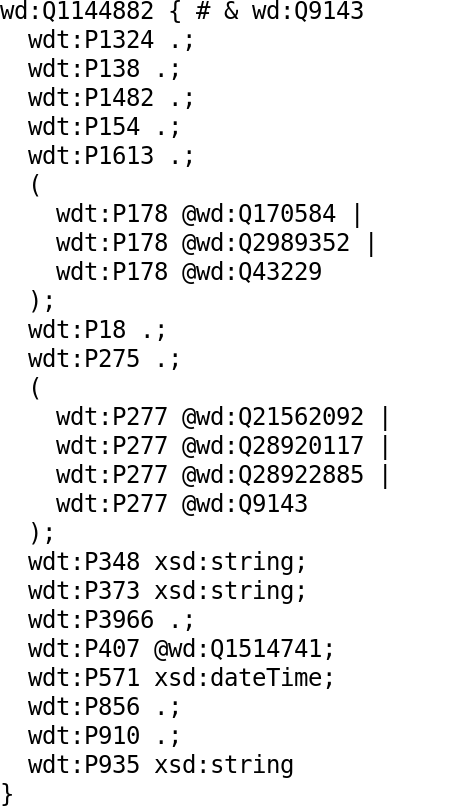
\includegraphics[trim={0 2.5cm 0 0},clip]{screenshots/shexc-no-syntax-highlighting}
    \caption{
      Excerpt of an inferred \gls{schema} for Linux distributions
    }
    \label{fig:shexc-syntax-highlighting-without}
  \end{subfigure}
  \begin{subfigure}[t]{0.45\textwidth}
    \centering
    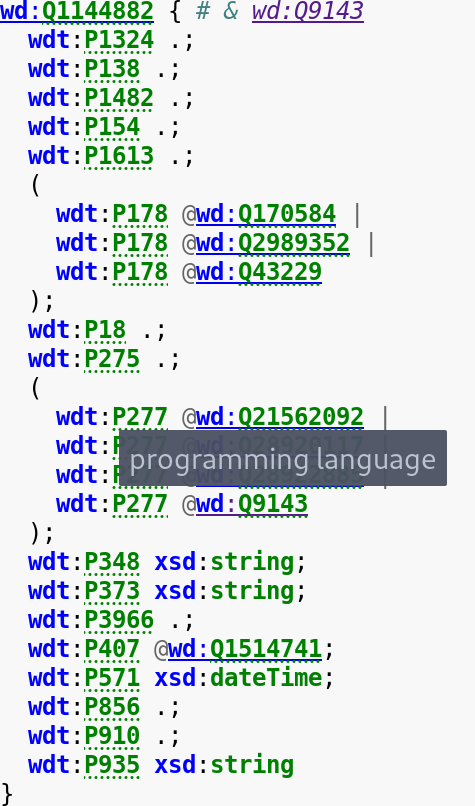
\includegraphics[trim={0 2.5cm 0 0},clip]{screenshots/shexc-with-syntax-highlighting}
    \caption[The same \gls{schema} with syntax highlighting and the script applied]{
      The same \gls{schema} with syntax highlighting and the script applied –
      the cursor is over the \lstinline{P277} \gls{property ID}
    }
    \label{fig:shexc-syntax-highlighting-with}
  \end{subfigure}
  \caption{
    Screenshots showing the effects of syntax highlighting and the client-side script
  }
  \label{fig:shexc-syntax-highlighting}
\end{figure}

\section{Toolforge Support}
\label{sec:wdsi:Toolforge}

Since Wikimedia Toolforge runs on a rather old Linux distribution
(Ubuntu 14.04 “Trusty Tahr”, originally released April 2014),
the versions of various software used by \gls{RDF2Graph} and the rest of the inference process
were too outdated to use out-of-the-box.
The response to this was twofold:
to cope with older software versions where feasible,
and to install newer software versions where not.

\Gls{RDF2Graph} required Java 8,
but only Java 7 is installed on Toolforge.
Fortunately, \gls{RDF2Graph} only used Java 8 for syntactic constructs (“lambda” syntax)
and those only sparingly, so it was not too much work to make it compatible with Java 7 again.
Similarly, Apache Jena and Fuseki have required Java 8 for some time already,
but fortunately \gls{RDF2Graph} is compatible with their older versions which support Java 7,
and which could therefore be installed.

On the other hand, there is no obvious way to make the \command{jq}-based part of the data download step
work with \command{jq} version 1.4, which has no general string replacement capabilities.
Therefore, \command{jq} version 1.5 was installed locally into the tool’s home directory –
as was the latest version of \gls{Node.js}, which was similarly outdated.
(The Pygments syntax highlighter mentioned in \cref{sec:wdsi:utilities} was also installed locally,
since \gls{shexc} syntax support is not yet available in any released version.)

Full installation instructions may be found in the \filename{README} file of the source code repository.

%% LaTeX2e class for student theses
%% sections/evaluation.tex
%% 
%% Karlsruhe Institute of Technology
%% Institute for Program Structures and Data Organization
%% Chair for Software Design and Quality (SDQ)
%%
%% Dr.-Ing. Erik Burger
%% burger@kit.edu
%%
%% Version 1.3.3, 2018-04-17

\chapter{Evaluation}
\label{ch:Evaluation}

The evaluation of this thesis
mainly focuses on the quality and usefulness of the resulting \glspl{schema}.
Unfortunately, without being able to reliably validate data sets against \glspl{schema} –
for example, to verify whether an \gls{item} for an author
matches a \gls{schema} inferred from fifty other authors –
it is not possible to objectively assess the quality of the inferred \glspl{schema}.
However, inspecting the \glspl{schema} manually
can still give insights on their quality (\cref{sec:Evaluation:quality}),
as well as the quality of the underlying data,
and it is also possible to extract smaller subsets from the full \glspl{schema},
which can then be used for validation (\cref{sec:Evaluation:extraction}).
In these ways, the \glspl{schema} can still be useful even though they can’t be used for validation directly.
Additionally, the runtime of the inference process is examined in \cref{sec:Evaluation:duration}.

\section{Schema Quality}
\label{sec:Evaluation:quality}

While the \gls{schema} quality cannot be assessed objectively without reliable validation,
it is possible to simply look at the \glspl{schema} and see if they “make sense” on their own.
Generally, the inferred \glspl{schema} are much too large to read the entire \gls{schema},
but one can select the \glspl{shape} for individual classes
(randomly or by searching for the \glspl{item ID} of specific classes)
and check their type links.
For example, \cref{listing:13th-riigikogu-Q5} shows the \gls{shape} for the class \QL{Q5}{human}
from the \gls{schema} inferred from 50 members of the 13th Riigikogu (the Estonian parliament).
In textual form, it means that a human should have the following \glspl{statement}:
\begin{itemize}
\item Member of any number of political parties, where the values are political parties.
\item Any number of occupations, where the values are positions.
  This likely reflects the fact that the input data only contained politicians –
  other \glspl{schema} often include other possible classes for this property,
  such as “occupation” or “profession”.
\item Any number of spoken, written or signed languages, where the values are languages.
\item Optionally, a name in the subject’s native language.
\item Any number of awards received, where the values are classes of awards.
  The target class, “class of award”, is an artifact of the not completely consistent modeling of awards in \gls{Wikidata}:
  there is sometimes confusion about the relationship between different “levels” of awards,
  such as “award”, “peace prize”, “Nobel Prize”, “Nobel Peace Prize”, “2018 Nobel Peace Prize”,
  and whether they should be instances or subclasses of each other.
\item Optionally, a place of birth, where the value is a human settlement.
\item Optionally, a sex or gender, where the value is a sex of humans or a gender.
  The two target classes are the result of the two most common gender \glspl{item} in \gls{Wikidata},
  \QL{Q6581097}{male} and \QL{Q6581072}{female},
  each having several \PL{P31}{instance of} statements.
\item Optionally, a country of citizenship, where the value is a political territorial entity.
\item Optionally, a \gls{Wikimedia Commons} category.
\item Any number of positions held by the subject, where the values are positions.
\item Optionally, a date of birth.
\item Any number of places where the subject was educated, where the values are educational institutions.
\item Optionally, a family name, where the value is a family name.
\item Optionally, a given name, where the value is a given name.
\item Any number of work locations, where the values are human settlements.
\end{itemize}

\begin{lstfloat}[t]
\begin{lstlisting}[language=sparql]
wd:Q5 { # & wd:Q215627
  wdt:P102 @wd:Q7278*;
  wdt:P106 @wd:Q4164871*;
  wdt:P1412 @wd:Q34770*;
  wdt:P1559 rdf:langString?;
  wdt:P166 @wd:Q38033430*;
  wdt:P19 @wd:Q486972?;
  (
    wdt:P21 @wd:Q4369513? |
    wdt:P21 @wd:Q48277?
  );
  wdt:P27 @wd:Q1048835?;
  wdt:P373 xsd:string?;
  wdt:P39 @wd:Q4164871*;
  wdt:P569 xsd:dateTime?;
  wdt:P69 @wd:Q2385804*;
  wdt:P734 @wd:Q101352?;
  wdt:P735 @wd:Q202444?;
  wdt:P937 @wd:Q486972*
}
\end{lstlisting}
\caption{Excerpt of a \gls{schema} inferred from 50 members of the 13th Riigikogu.}
\label{listing:13th-riigikogu-Q5}
\end{lstfloat}

Aside from some quirks of the input data, all of these seem reasonable to me.
The most obvious missing \glspl{predicate} are date and place of death,
which is again due to the input data set:
all the members of the current Estonian parliament are alive,
and while one might expect to see dates of death on some \glspl{item} they link to,
the fact that currently only 33 parents of members of the 13th Riigikogu are known to \gls{Wikidata}
makes it seem plausible enough that there simply happened to be no dead humans in the full input data.

As the input data sets get larger,
the \glspl{schema} also tend to grow:
in the number of \glspl{shape} (classes),
the number of \glspl{predicate} in each \gls{shape},
and also in the number of possible classes for a predicate.
For example, before simplification,
the \QL{Q5}{human} \gls{shape} from the \gls{schema} inferred from the set of US presidents
lists \emph{nine} possible classes for someone’s \PL{P735}{given name}:
\begin{itemize}
\item A generic \QL{Q202444}{given name},
  such as \QL{Q18396847}{Boylston} in Thomas Boylston Adams, the third son of President John Adams.
  (The more common given names generally have a more specific class,
  usually one of the next three listed here.)
\item A \QL{Q12308941}{male given name},
  such as \QL{Q677191}{James} in President James A.~ Garfield.
\item A \QL{Q11879590}{female given name},
  such as \QL{Q644599}{Ida} in Ida Stover Eisenhower, mother of President Eisenhower.
\item A \QL{Q3409032}{unisex given name},
  such as \QL{Q564684}{Anne} in Nancy Reagan (born Anne Frances Robbins), wife of President Reagan.
  (“Anne” is a female given name in English,
  but sometimes used as a male given name in the Netherlands or France,
  and therefore classified as both female and unisex in \gls{Wikidata}, depending on language.)
\item A \QL{Q1243157}{compound given name},
  such as \QL{Q16275947}{George Washington} in George Washington Adams, the first son of President John Quincy Adams.
\item A \QL{Q1130279}{hypocorism} (a diminutive form of a name),
  such as \QL{Q2165388}{Ron} in Ron Reagan, son of President Reagan.
\item A \QL{Q108709}{diminutive},
  such as \QL{Q4166211}{Jimmy} in President Jimmy Carter.
  Arguably, that \gls{item} should be an instance of the aforementioned hypocorism class
  instead of the more generic diminutive class, which also includes non-names like “auntie”.
\item \QL{Q19803443}{Initials instead of given names},
  such as \QL{Q19803518}{S.} in President Harry S.~Truman (not an abbreviation).
\item A \QL{Q101352}{family name},
  such as \QL{Q2800825}{Simpson} in President Ulysses S.~Grant
  (the “S.” is sometimes believed to be short for “Simpson”, his mother’s maiden name).
  This is clearly an error: even if the “S.” does stand for “Simpson”, which Grant denied,
  the correct \gls{item} to use would be the given name \Q{Q50876620}, not the family name \Q{Q2800825}.
\end{itemize}

If the problems pointed out above were to be fixed,
all the remaining classes could be merged into the generic \QL{Q202444}{given name} class,
as in the earlier \gls{schema}.
However, due to the presence of \QL{Q101352}{family name},
the best common superclass is instead \QL{Q10856962}{anthroponym},
the common superclass of given and last names,
and the \QL{Q108709}{diminutive} class remains unmerged,
as it is not a subclass of any kind of name.

One can continue to pick apart the generated \glspl{schema} in this manner for hours,
and I have done so while working on this thesis
in order to find problems and possible improvements in the inference process.
Three insights emerge:

\begin{enumerate}
\item The simplification step is vital for readable \glspl{schema}.
  The \glspl{schema} are no less correct without simplification as far as the input data set is concerned,
  but if the numerous subclasses in \gls{Wikidata}’s hierarchy are never merged,
  the \glspl{schema} become exceedingly tedious to read for humans,
  and they will also often match other data sets less well
  if the other data sets involve subclasses that were not encountered in the original input data.

  This can be seen in some of the older \glspl{job} of the \gls{wdsi}:
  if there is a \lstinline[language=java]{StackOverflowError} in the standard error of the inference process,
  it means that \gls{RDF2Graph} crashed during the simplification step
  and the \gls{shex} export ran on the original, unsimplified graph.
  (Later, the inference step was made more robust,
  which is why newer \glspl{job} do not have this problem.)

\item Sometimes, biases in the \gls{schema} are visible, due to biases in the input data set.
  (In one particularly egregious case,
  a \gls{schema} proclaimed that a given name must always be a \emph{male} given name,
  since there had been no women with given names in the input data set.)
  One can presume that at other times biases in the \gls{schema} are not visible,
  which does not mean that they are not present. % TODO abbreviate to “not visible, but still present”?
  To arrive at useful \glspl{schema},
  care must be taken when selecting the input data set,
  and the results must be viewed critically. % TODO is “viewed” the best verb here?

\item Sometimes, the \gls{schema} reflects errors in the input data,
  as in the case above where a family name \gls{item} was used for a given name.
  This can often be traced back to confusion between several \glspl{item} with similar labels.
  Such errors are usually visible in the resulting \gls{schema} if one takes the time to read it,
  though they are not always obvious due to the simplification
  (as when the classes for given and family names were merged into anthroponyms above).
\end{enumerate}

\section{Manual Schema Extraction}
\label{sec:Evaluation:extraction}

One way to make use of the inferred \glspl{schema}
even though they cannot be used for validation directly
is to extract a smaller subset of the \gls{schema} manually,
then validating \glspl{item} against that.
If desired, that \gls{schema} can then be further altered and augmented as deemed necessary,
making the original \gls{schema} the basis of a manually curated one.

Generally, to extract parts of the \gls{schema},
one starts with a basic \gls{shape} for the input \glspl{item}
(e.~g. \QL{Q5}{human} if the \gls{schema} was inferred from a set of humans),
copies it into the reduced \gls{schema},
and repeats this procedure for all \glspl{shape} (classes) mentioned by that \gls{shape} which had not been copied yet.
\Glspl{predicate} which link to \glspl{shape} that should not be included can be dropped when copying a \gls{shape}:
for example, the \PL{P27}{country of citizenship} \gls{shape} should be dropped
if one is not interested in including \glspl{shape} for countries, states etc. in the reduced \gls{schema}.
Some \glspl{predicate} may also need to be moved between \glspl{shape},
or the target classes may need to be adjusted,
if the results of the automatic simplification are not satisfactory,
e.~g. if unrelated classes were merged into a very fundamental base class like \QL{Q937228}{property}
despite the changes in \cref{subsec:RDF2Graph+Wikidata:Wikidata:simplification}.

\begin{lstfloat}[ht]
\begin{sublstfloat}[t]{0.45\textwidth}
\begin{lstlisting}[language=sparql,showlines=true]
wd:Q12136 {
  wdt:P1478 @wd:Q16521?;
  wdt:P1748 xsd:string?;
  wdt:P2572 xsd:string?;
  wdt:P373 xsd:string?;
  wdt:P667 xsd:string?;
  wdt:P828 @wd:Q16521?
}

wd:Q16521 {
  wdt:P1542 @wd:Q12136?;
  wdt:P171 @wd:Q16521*;
  wdt:P225 xsd:string?;
  wdt:P373 xsd:string?;
  wdt:P935 xsd:string?
}
















\end{lstlisting}
\caption{Schema for diseases, based on \wdsiJob{37}.}
\label{listing:zika}
\end{sublstfloat}
\begin{sublstfloat}[t]{0.45\textwidth}
\begin{lstlisting}[language=sparql]
wd:Q11424 {
  wdt:P1040 @wd:Q5*;
  wdt:P1431 @wd:Q5*;
  wdt:P154 .?;
  wdt:P161 @wd:Q5*;
  wdt:P162 @wd:Q5*;
  wdt:P175 @wd:Q5?;
  wdt:P1809 @wd:Q5*;
  wdt:P2130 xsd:decimal?;
  wdt:P2142 xsd:decimal?;
  wdt:P2515 @wd:Q5*;
  wdt:P2554 @wd:Q5*;
  wdt:P2769 xsd:decimal?;
  wdt:P3092 @wd:Q5*;
  wdt:P3174 @wd:Q5*;
  wdt:P3300 @wd:Q5?;
  wdt:P344 @wd:Q5*;
  wdt:P373 xsd:string?;
  wdt:P57 @wd:Q5*;
  wdt:P58 @wd:Q5*;
  wdt:P725 @wd:Q5*;
  wdt:P86 @wd:Q5*
}

wd:Q5 {
  wdt:P22 @wd:Q5?;
  wdt:P25 @wd:Q5?;
  wdt:P26 @wd:Q5*;
  wdt:P40 @wd:Q5*;
  wdt:P569 xsd:dateTime?;
  wdt:P570 xsd:dateTime?
}
\end{lstlisting}
\caption{Schema for films, based on \wdsiJob{36}.}
\label{listing:films}
\end{sublstfloat}
\caption{Two \glspl{schema} manually extracted from automatically inferred ones.}
\label{listing:extracted}
\end{lstfloat}

\Cref{listing:extracted} shows two \glspl{schema} that were manually extracted in this fashion
from \glspl{schema} inferred by the \gls{wdsi}.
\Cref{listing:zika} was extracted from a \gls{schema}
inferred from 100 scientific articles about the Zika virus,
and contains \glspl{shape} for the classes \QL{Q12136}{disease} and \QL{Q16521}{taxon}:
diseases may be caused (indirectly or immediately) by taxa,
and taxa may effect diseases and have any number of parent taxa.
\Cref{listing:films} was extracted from a \gls{schema}
inferred from the set of films which won three or more Academy Awards (“Oscars”) % TODO glossary? ™?
and contains \glspl{shape} for the classes \QL{Q11424}{film} and \QL{Q5}{human}:
films have human directors, editor, cast members, screenwriters, etc.,
and humans may have parents, any number of spouses and children, and dates of birth and death.

These \glspl{schema} are simple enough that they can be validated using the “Simple Online Validator”
at \url{https://rawgit.com/shexSpec/shex.js/wikidata/doc/shex-simple.html},
which automatically downloads all the required data from \gls{Wikidata}.
Validating 100 arbitrary diseases
against the \gls{shape} for \QL{Q12136}{disease} from \cref{listing:zika} mostly yields positive results,
with only four violations:
the \glspl{item} \QL{Q366964}{X-linked adrenoleukodystrophy},
\QL{Q580285}{Morquio Syndrome} and \QL{Q2200359}{Sanfilippo syndrome}
have more than one \PL{P1748}{NCI Thesaurus ID} \gls{statement}, while the \gls{schema} says a disease may only have zero or one such IDs,
and the \gls{item} \QL{Q895930}{nodding disease} fails validation because it has two \PL{P828}{has cause} \glspl{statement},
\QL{Q8084905}{autoimmune disease} and \QL{Q1601794}{parasitic infectious diseases},
whereas the \gls{schema} says a disease may only have zero or one causes.
(The \gls{schema} also says that those causes should be taxa, not other diseases,
but the \gls{shape} for taxa is sufficiently lax that these diseases match it.)
Validating 100 arbitrary films
against the \gls{shape} for \QL{Q11424}{film} from \cref{listing:films} also yields positive results with only a single violation –
\QL{Q185143}{Detective Conan} has two \PL{P154}{logo image} \glspl{statement} (French and Japanese)
whereas the \gls{schema} says it should only have one.

A second look at the \glspl{schema} makes it clear why there are so few violations:
the cardinalities for all \glspl{predicate}, without exception,
are either \lstinline{?} (“zero or one”) or \lstinline{*} (“any number”).
A completely empty \gls{item} with no \glspl{statement} at all
will match all four \glspl{shape} in \cref{listing:extracted}.
This is likely an artifact of the \gls{schema} extraction procedure,
which in this case was extremely selective of \glspl{shape}
to ensure that the \gls{schema} would fit on one page of this document,
and therefore only included very few \glspl{shape},
each of which had had a high number of examples in the input data set:
enough that, for any \gls{property},
there was an example \gls{item} missing \glspl{statement} for that \gls{property},
forcing the lower boundary of the cardinality to be zero.
Overall, the sample \glspl{schema} investigated in \cref{sec:jobs-over-various}
have \SIrange{17}{34}{\percent} of non-optional \glspl{predicate},
so if one includes some more \glspl{shape} during the extraction process,
they are bound to include some required \glspl{predicate} soon.
(Alternatively, the cardinality of some \glspl{predicate} could be manually raised during the extraction.)

Generally, these extracted \glspl{schema} appear to be useful to find some mistakes,
though their utility can be increased by extracting larger parts of the \glspl{schema}
and by further refining them according to one’s personal experience with the data model.
A useful side effect is that the kind of careful inspection of the \gls{schema}
which is necessary to extract useful parts of it
will also likely find some problems in the \gls{schema} where they exist,
pointing at errors in the original input data set,
as demonstrated in \cref{sec:Evaluation:quality}.

\section{Duration of the Inference Process}
\label{sec:Evaluation:duration}

While attempts to validate data against the inferred \gls{schema}
suffer due to the size of the input data and the \glspl{schema},
no such problems appear to plague the inference process,
which, while slow, has a more reliable runtime.
To some degree, this was already apparent in the execution times
of the various \glspl{job} that were run on the \gls{wdsi}:
ranging from five or ten minutes to several hours,
they roughly follow the size of the input data linearly.

However, the timing data from the \gls{wdsi}
is not without its problems:
as the tool was tested with different \glspl{job},
various problems were discovered and subsequently fixed
(some of them described in more detail earlier, others too minor to be worth mentioning),
so the runtimes available from the tool apply to a range of software versions,
with several instances of the same \gls{job} being repeated (to verify a software fix)
with highly different runtimes.
Therefore, a subset of the tool’s \glspl{job} was selected
and repeated locally, with a single software version,
to get more reliable execution times.
\Cref{sec:jobs-over-various} contains graphs of runtime over various factors,
which are explained in more detail in the following paragraphs,
each with three different functions fitted to the data:
a simple linear function $a+bx$,
a quadratic function $a+bx+cx^2$,
and a power function $a+bx^c$.
Each figure contains two subfigures,
one for the full data and one with two outlier records removed –
see the text in the appendix for details.

The most obvious possible relation is
to directly compare the runtime to the number of \glspl{item} selected by the user’s query,
as shown in \cref{fig:jobs-over-entities}.
However, it is clear from the graphs that there is no direct relation
between the number of \glspl{item} and the runtime:
in fact, four of the six resulting functions suggest that
execution time shall become negative if one only supplies enough \glspl{item},
which is clearly nonsensical.
This is not surprising,
because the amount of work that \gls{RDF2Graph} has to do
highly depends on the size of the \glspl{item},
as well as the number of \glspl{item} indirectly selected as the values of \glspl{statement} on the original \glspl{item} (and their size).

Instead, a much more sensible relation is the total amount of input data:
the number of \glspl{triple} which Fuseki serves to \gls{RDF2Graph}
(that is, the number of lines in the \gls{N-Triples} file).
As can be seen in \cref{fig:jobs-over-triples},
this results in a fairly linear relation,
especially if two outliers are removed,
in which case the functions fit the data very well.
However, with the outliers included the fit is much less satisfactory.

\begin{lstfloat}[b]
\begin{lstlisting}[language=awk]
BEGINFILE {
  count = 0;
}

$2 == "<http://www.wikidata.org/prop/direct/P31>" {
  count++;
}

ENDFILE {
  print FILENAME, count
}
\end{lstlisting}
\caption{GNU AWK script to count the number of \PName{wdt:P31} triples in the input.}
\label{listing:P31}
\end{lstfloat}

\begin{lstfloat}[b]
\begin{lstlisting}[language=awk]
BEGINFILE {
  count = 0;
  delete classes;
}

$2 == "<http://www.wikidata.org/prop/direct/P31>" {
  classes[$3]++
}

ENDFILE {
  for (class in classes)
    count++;
  print FILENAME, count;
}
\end{lstlisting}
\caption{GNU AWK script to count distinct classes in the input.}
\label{listing:classes}
\end{lstfloat}

Since \gls{RDF2Graph} heavily relies on type information,
another possible factor for execution time
is just the number of \PName{wdt:P31} \glspl{triple} in the input,
rather than the overall number of \glspl{triple}.
(Recall that \PL{P31}{instance of} is the \gls{Wikidata} property linking an \gls{item} to its class.)
% TODO a) is that “recall” appropriate? b) was that even clearly explained yet?
The number of \PName{wdt:P31} \glspl{triple} was counted
using the GNU AWK snippet found in \cref{listing:P31},
and the result is shown in \cref{fig:jobs-over-P31s}:
the functions are more linear and fit the data better, both with and without outliers.
However, with outliers included the fit is still not completely satisfactory.

Alternatively, instead of counting \PName{wdt:P31} \glspl{triple}
it is also possible to count the distinct number of classes in the input data.
Classes were counted using the GNU AWK snippet found in \cref{listing:classes},
and the result is shown in \cref{fig:jobs-over-classes}:
the functions are significantly less linear now
(though this is not visible in the function equations shown in the graphs, due to rounding),
but they finally fit the data well without excluding the outliers:
in fact, the graph with outliers has slightly better fits than the one without outliers.

Two conclusions are possible from this:
the execution time could derive linearly from the number of input \gls{triple} or \PName{wdt:P31} \gls{triple},
or it could derive nonlinearly from the number of input classes.
The first conclusion has no satisfactory explanation for the outliers
which need to be excluded to get good function fits,
whereas the second conclusion requires no cherry-picking in the data
but lacks an explanation for the nonlinear runtime.
% TODO is this undecidedness between the conclusions acceptable?

One might think that these relations are not very useful
because they only predict the duration of the whole process partway through the process.
However, all of the possible predictor variables – % TODO “predictor variables” feels weird – regressors? independent variables?
number of \glspl{item}, number of \glspl{triple}, number of \PName{wdt:P31} \glspl{triple}, number of distinct classes –
can be determined after the data download step,
which is both the very first step in the whole process
and also does not take a long time:
in the jobs listed in \cref{sec:jobs-over-various},
the download never takes more than twenty seconds,
and for most jobs it finishes within about five seconds.
This means that it takes less than half a minute
to be able to mostly predict the duration of the full \gls{job}, which can be several hours.
This suggests two possible future improvements
for the \gls{wdsi}:
to report to the user how long a \gls{job} is expected to take,
as soon as the download step has finished;
and to reject \glspl{job} which resulted in too much data,
and are expected to take far too long to be tolerable.
Currently, the tool merely suggests to its users
that their queries should not select more than about fifty \glspl{item},
but does not implement any kind of hard limit beyond that.

%% LaTeX2e class for student theses
%% sections/conclusion.tex
%% 
%% Karlsruhe Institute of Technology
%% Institute for Program Structures and Data Organization
%% Chair for Software Design and Quality (SDQ)
%%
%% Dr.-Ing. Erik Burger
%% burger@kit.edu
%%
%% Version 1.3.3, 2018-04-17

\chapter{Conclusion}
\label{ch:Conclusion}

The goal of this thesis was to investigate how \gls{shex} \glspl{schema} can be automatically inferred for \gls{Wikidata},
and how useful the resulting \glspl{schema} are.
This was done using an updated and adapted version of the \gls{RDF2Graph} software,
which was made available to the \gls{Wikidata} community
through a new web-based tool.

In addition to the changes specific to \gls{Wikidata},
many general improvements to \gls{RDF2Graph} were made over the course of this thesis,
making it easier to use and more robust on any graph.
All these changes are available under the same free software license as the original \gls{RDF2Graph},
and I hope that some of them will be included in the original source code repository in the future.

When attempting to validate other \glspl{item} against the inferred \glspl{schema},
an unexpected problem arose:
none of the existing \gls{shex} validators were able to reliably perform the validation without crashing.
Several strategies were attempted to remediate this,
both in the \gls{schema} extraction and in the validators,
but this was ultimately unsuccessful.

However, this does not mean the \glspl{schema} are not useful.
Sometimes, problems in the input data can manifest themselves
in the form of unusual \glspl{predicate} or target classes in a \gls{schema},
which an attentive reader can notice and trace back to the problematic \glspl{item} in the input.
And the full, automatically inferred \glspl{schema}
can also form the basis for shorter \glspl{schema} manually extracted from the longer ones,
which can either be validated directly
(now without problems from the validators)
or be further refined by users familiar with the data model,
making the automatically inferred \glspl{schema} a useful basis for manually curated \glspl{schema}.

There are plenty of options of further improvements on this work.
\Cref{sec:Evaluation:duration} already mentioned how the \gls{wdsi} could be improved
to notify the user of the estimated total runtime of a \gls{job} once the data download step is complete
and to reject \glspl{job} which are expected to take too long.
Many other improvements could be made to the user interface as well,
such as exposing some more configuration options to users of the tool,
e.~g. the thresholds for \gls{schema} reduction mentioned in \cref{sec:RDF2Graph+Wikidata:schema-reduction}.

A significant improvement over the current state
would be to make \gls{RDF2Graph} work on full \gls{statement} nodes instead of just the “truthy” \glspl{statement}.
A full explanation of full \gls{statement} nodes is beyond the scope of this thesis,
but in brief, they offer much more information about \gls{Wikidata} \glspl{statement}
in exchange for a slightly more complicated data format.
Using full \gls{statement} nodes would allow \gls{RDF2Graph} to take not just the \gls{statement}’s values
but also their \glspl{qualifier} and \glspl{reference} into account.
However, this would require major changes to the way \gls{RDF2Graph} looks at the input graph,
because the \gls{subject} and \gls{object} of a \gls{statement} are no longer linked via a single \gls{triple}
in the full \gls{statement} nodes.

Clearly, it is not a satisfactory final state
that the inferred \glspl{schema} cannot be directly used for validation.
It may be possible to find optimizations in the validators
and/or useful criteria for reducing the inferred \glspl{schema}
which would enable direct validation against the \glspl{schema}
without human intervention to manually extract their most useful parts.
There is also some room for improvement in the simplification step
regardless of the ability to validate against the inferred \glspl{schema}:
sometimes, despite the changes in \cref{subsec:RDF2Graph+Wikidata:Wikidata:simplification},
it still merges mostly-unrelated classes into very abstract base classes,
so the criteria on when to merge or not merge classes could use some improvements.
It may also be useful to apply some of the thresholds for schema reduction (\cref{sec:RDF2Graph+Wikidata:schema-reduction})
before the simplification step starts,
so that, for instance,
a \gls{type link} of \QL{Q101352}{family name} for the \PL{P735}{given name} \gls{predicate}
is filtered out before it is merged with \QL{Q202444}{given name} into \QL{Q10856962}{anthroponym} in simplification.

The detailed timings for the jobs listed in \cref{sec:jobs-over-various}
show that the \gls{shex} export step usually takes up about half of the total wall-clock time,
and often significantly more than half of the CPU time.
This thesis does not investigate this step more closely except for its very last part
(see \cref{sec:RDF2Graph+Wikidata:updates}),
but it seems unlikely that this is necessary:
it may be possible to change or rewrite the rest of the \gls{shex} exporter to be much more efficient.

% TODO finish off conclusion?


%% --------------------
%% |   Bibliography   |
%% --------------------

%% Add entry to the table of contents for the bibliography
\printbibliography[heading=bibintoc]

%% --------------------
%% |   Glossary       |
%% --------------------

\printglossaries

%% ----------------
%% |   Appendix   |
%% ----------------
\appendix
%% LaTeX2e class for student theses
%% sections/apendix.tex
%% 
%% Karlsruhe Institute of Technology
%% Institute for Program Structures and Data Organization
%% Chair for Software Design and Quality (SDQ)
%%
%% Dr.-Ing. Erik Burger
%% burger@kit.edu
%%
%% Version 1.3.3, 2018-04-17

\iflanguage{english}
{\chapter{Appendix}}    % english style
{\chapter{Anhang}}      % german style
\label{chap:appendix}

\section{Results of Validation With Depth Limit}
\label{sec:appendix:depth-limit}

The following tables show the results
when attempting various validations against inferred \glspl{schema}
with different depth limits.
The meaning of the result column is as follows:

\begin{description}
\item[solved] validation completed successfully (found a solution)
\item[fail] validation completed unsuccessfully (reported violations)
\item[limit] the result is directly “depth limit reached” % TODO perhaps just remove these lines?
\item[core] the process crashed and dumped core (out-of-memory error)
\item[abort] the process was manually killed after a long time with no apparent progress
\end{description}

\begin{table}[ht]
  \centering
  \begin{tabular}{r r r l}
    limit & real time & CPU time & result \\
    \hline
    - & \minsec{2}{50} & \minsec{8}{51} & core \\
    1 & \minsec{0}{0} & \minsec{0}{0} & limit \\
    2 & \minsec{4}{41} & \minsec{17}{22} & core \\
    3 & \minsec{3}{57} & \minsec{13}{31} & core \\
    4 & \minsec{2}{51} & \minsec{9}{1} & core \\
    5 & \minsec{2}{48} & \minsec{8}{54} & core \\
    6 & \minsec{2}{50} & \minsec{8}{58} & core \\
    7 & \minsec{2}{48} & \minsec{8}{41} & core \\
    8 & \minsec{2}{47} & \minsec{8}{44} & core \\
    9 & \minsec{2}{48} & \minsec{8}{48} & core \\
    10 & \minsec{2}{48} & \minsec{8}{53} & core
  \end{tabular}
  \caption{
    Results when validating the \gls{item} \QL{Q44578}{Titanic}
    against the \gls{shape} for the class \QL{Q11424}{film}
    from a \gls{schema} inferred from the set of films that won ten or more Oscars
    (\wdsiJob{29})
  }
  \label{tab:appendix:depth-limit:1}
\end{table}

\begin{table}[ht]
  \centering
  \begin{tabular}{r r r l}
    limit & real time & CPU time & result \\
    \hline
    - & \minsec{0}{1} & \minsec{0}{3} & fail \\
    1 & \minsec{0}{0} & \minsec{0}{0} & limit \\
    2 & \minsec{0}{16} & \minsec{0}{21} & core \\
    3 & \minsec{0}{1} & \minsec{0}{2} & fail \\
    4 & \minsec{0}{1} & \minsec{0}{3} & fail \\
    5 & \minsec{0}{1} & \minsec{0}{3} & fail \\
    6 & \minsec{0}{1} & \minsec{0}{3} & fail \\
    7 & \minsec{0}{1} & \minsec{0}{3} & fail \\
    8 & \minsec{0}{1} & \minsec{0}{2} & fail \\
    10 & \minsec{0}{1} & \minsec{0}{3} & fail
  \end{tabular}
  \caption{
    Results when validating the \gls{item} \QL{Q42}{Douglas Adams}
    against the \gls{shape} for the class \QL{Q5}{human}
    from a \gls{schema} inferred from the set of films that won ten or more Oscars
    (\wdsiJob{29})
  }
  \label{tab:appendix:depth-limit:2}
\end{table}

\begin{table}[ht]
  \centering
  \begin{tabular}{r r r l}
    limit & real time & CPU time & result \\
    \hline
    - & \minsec{0}{17} & \minsec{0}{7} & fail \\
    1 & \minsec{0}{0} & \minsec{0}{0} & limit \\
    2 & \minsec{0}{0} & \minsec{0}{1} & solved \\
    3 & \minsec{0}{18} & \minsec{0}{7} & fail \\
    4 & \minsec{0}{19} & \minsec{0}{8} & fail \\
    5 & \minsec{0}{17} & \minsec{0}{7} & fail \\
    6 & \minsec{0}{18} & \minsec{0}{8} & fail \\
    7 & \minsec{0}{18} & \minsec{0}{8} & fail \\
    8 & \minsec{0}{18} & \minsec{0}{8} & fail \\
    9 & \minsec{0}{18} & \minsec{0}{7} & fail \\
    10 & \minsec{0}{18} & \minsec{0}{7} & fail
  \end{tabular}
  \caption{
    Results when validating the \gls{item} \QL{Q42}{Douglas Adams}
    against the \gls{shape} for the class \QL{Q5}{human}
    from a \gls{schema} inferred from the members of the 13th Riigikogu
    (the Estonian parliament; \wdsiJob{30})
  }
  \label{tab:appendix:depth-limit:3}
\end{table}

\begin{table}[ht]
  \centering
  \begin{tabular}{r r r l}
    limit & real time & CPU time & result \\
    \hline
    - & \minsec{2}{50} & \minsec{8}{51} & core \\
    1 & \minsec{0}{0} & \minsec{0}{0} & limit \\
    2 & \minsec{4}{41} & \minsec{17}{22} & core \\
    3 & \minsec{3}{57} & \minsec{13}{31} & core \\
    4 & \minsec{2}{51} & \minsec{9}{1} & core \\
    5 & \minsec{2}{48} & \minsec{8}{54} & core \\
    6 & \minsec{2}{50} & \minsec{8}{58} & core \\
    7 & \minsec{2}{48} & \minsec{8}{41} & core \\
    8 & \minsec{2}{47} & \minsec{8}{44} & core \\
    9 & \minsec{2}{48} & \minsec{8}{48} & core \\
    10 & \minsec{2}{48} & \minsec{8}{53} & core
  \end{tabular}
  \caption{
    Results when validating the \gls{item} \QL{Q449851}{Mailis Reps}
    against the \gls{shape} for the class \QL{Q5}{human}
    from a \gls{schema} inferred from the members of the 13th Riigikogu
    (\wdsiJob{30})
  }
  \label{tab:appendix:depth-limit:4}
\end{table}

\begin{table}[ht]
  \centering
  \begin{tabular}{r r r l}
    limit & real time & CPU time & result \\
    \hline
    - & \minsec{1}{25} & \minsec{4}{14} & core \\
    1 & \minsec{0}{1} & \minsec{0}{1} & limit \\
    2 & \minsec{0}{1} & \minsec{0}{1} & fail \\
    3 & \minsec{0}{55} & \minsec{2}{6} & core \\
    4 & \minsec{7}{34} & 1\minsec{3}{54} & core \\
    5 & \minsec{0}{10} & \minsec{0}{27} & core \\
    6 & \minsec{0}{30} & \minsec{1}{5} & core \\
    7 & \minsec{0}{51} & \minsec{1}{59} & core \\
    8 & \minsec{5}{29} & 1\minsec{2}{54} & core \\
    9 & \minsec{0}{9} & \minsec{0}{19} & core \\
    10 & 8\minsec{6}{39} & 15\minsec{3}{35} & abort
  \end{tabular}
  \caption{
    Results when validating the \gls{item} \QL{Q30}{United States of America}
    against the \gls{shape} for the class \QL{Q3624078}{sovereign state}
    from a \gls{schema} inferred from a set of \glspl{item} for bus stops
    (\wdsiJob{15})
  }
  \label{tab:appendix:depth-limit:5}
\end{table}

\section{Job Execution Times}
\label{sec:jobs-over-various}
% TODO section heading is currently separated from the graphs
% by some of the tables above

The following charts show the total execution time of the inference process
for various input queries collected from the \gls{wdsi}:

\begin{itemize}
\item Members of the 30th Riigikogu (the Estonian parliament),
  limited to 50 \glspl{item}.
  Originally \wdsiJob{30}.
\item The Federal Chancellors of Germany,
  originally \wdsiJob{1}.
\item Films that won three or more Academy Awards (“Oscars”). % glossary? ™?
  Originally \wdsiJob{32}, later repeated as \wdsiJob{34}, \wdsiJob{35}, \wdsiJob{36}.
  (Some earlier jobs used a similar query with a limit of ten or five Oscars.)
\item The human \glspl{item} with most \glspl{sitelink} to other \gls{Wikimedia} projects
  (including but not limited to \gls{Wikipedia} articles in different language editions),
  limited to 50 \glspl{item}.
  Originally \wdsiJob{24}, later repeated as \wdsiJob{26}, \wdsiJob{27}.

  This is one of the two outliers removed for the first version of each chart,
  since it has an unusually high execution time compared to the amount of input data.
  My best explanation for that is that this is a less “coherent” set of \glspl{item}:
  since the selection criterion (the number of sitelinks) is not directly related to the data,
  this includes politicians, authors, religious figures, scientists, philosophers, celebrities, composers, and other kinds of people
  (though none of these are \emph{classes} in the sense relevant to \gls{RDF2Graph}).
\item The largest cities in the world by population,
  limited to 25 \glspl{item}.
  Originally \wdsiJob{3}.
\item Mammal taxa (including species but also genera, families etc.).
  Limited to \num{20000} \glspl{item},
  a limit that was experimentally determined to produce a high but not exorbitant number of triples.
  Originally \wdsiJob{33}.

  This is the second of the two outliers removed for the first version of each chart,
  due to the absurd number of input \glspl{item}:
  compare especially the $X$-axes of
  \cref{fig:jobs-over-entities-with-outliers,fig:jobs-over-entities-without-outliers}.
\item Programming languages with the highest number of \glspl{statement},
  limited to 50 \glspl{item}.
  Originally \wdsiJob{17}, later repeated as \wdsiJob{18}.
\item Recently edited \glspl{item} for \glspl{rfc},
  limited to 500 \glspl{item}.
  Originally \wdsiJob{21}, based on the earlier \wdsiJob{20} (equivalent but with a lower limit),
  which in turn was inspired by \wdsiJob{8}.
\item The member states of the United Nations, % TODO acronym?
  originally \wdsiJob{23}.
\item The presidents of the United States of America,
  originally \wdsiJob{2}.
\item The chapter organizations of the \gls{Wikimedia} Foundation, % TODO separate entry for WMF?
  originally \wdsiJob{5}.
\end{itemize}

For each input query,
the different steps of the inference process
(data download, initial \gls{RDF2Graph} run, \gls{RDF2Graph} simplification, \gls{shex} export)
were timed individually,
recording the real (“wall-clock”) time, user CPU time and system CPU time separately.
Only the sum of the real time was used for the charts below,
but the full data is available in the source code repository for this thesis.
% TODO okay to mention the repository? if yes, dump its url somewhere!
All the steps were performed on a system
with an Intel® Core™ i7-4771 CPU (\SI{3.50}{\giga\hertz} clock rate),
% TODO the ® and ™ are taken from the /proc/cpuinfo output, but I’m not sure if they’re necessary or just look stupid tbh
ca. \SI{25.2}{\giga\byte} (\SI{23.5}{\gibi\byte}) of memory,
and a network connection allowing download rates of up to \SI{23.6}{\mebi\byte\per\second} from \gls{wdqs},
with no significant other load of any kind at the time of measurement.

In addition to the graphs shown here,
the full data also shows that the simplification step of the process
never takes more than a minute,
which means that while the changes in \cref{sec:RDF2Graph+Wikidata:cyclic-graphs} potentially slowed this step down to some degree,
it does not make a big difference for the total execution time,
which is mostly dominated by other steps
(\gls{RDF2Graph} without simplification and \gls{shex} export)
anyways.

\begin{figure}[ht]
  \begin{subfigure}{\textwidth}
    \centering
    \input{graphs/jobs-over-entities}
    \caption{Job execution time over number of \glspl{item}, with outliers}
    \label{fig:jobs-over-entities-with-outliers}
  \end{subfigure}
  \begin{subfigure}{\textwidth}
    \centering
    \input{graphs/jobs-without-outliers-over-entities}
    \caption{Job execution time over number of \glspl{item}, without outliers}
    \label{fig:jobs-over-entities-without-outliers}
  \end{subfigure}
  \caption{Job execution time over number of \glspl{item} selected by the query}
  \label{fig:jobs-over-entities}
\end{figure}

\begin{figure}[ht]
  \begin{subfigure}{\textwidth}
    \centering
    \input{graphs/jobs-over-triples}
    \caption{Job execution time over number of \glspl{triple}, with outliers}
    \label{fig:jobs-over-triples-with-outliers}
  \end{subfigure}
  \begin{subfigure}{\textwidth}
    \centering
    \input{graphs/jobs-without-outliers-over-triples}
    \caption{Job execution time over number of \glspl{triple}, without outliers}
    \label{fig:jobs-over-triples-without-outliers}
  \end{subfigure}
  \caption{Job execution time over number of \glspl{triple} in the input data set}
  \label{fig:jobs-over-triples}
\end{figure}

\begin{figure}[ht]
  \begin{subfigure}{\textwidth}
    \centering
    \input{graphs/jobs-over-P31s}
    \caption{Job execution time over number of \PName{wdt:P31} \glspl{triple}, with outliers}
    \label{fig:jobs-over-P31s-with-outliers}
  \end{subfigure}
  \begin{subfigure}{\textwidth}
    \centering
    \input{graphs/jobs-without-outliers-over-P31s}
    \caption{Job execution time over number of \PName{wdt:P31} \glspl{triple}, without outliers}
    \label{fig:jobs-over-P31s-without-outliers}
  \end{subfigure}
  \caption{Job execution time over number of \PName{wdt:P31} \glspl{triple} in the input data set}
  \label{fig:jobs-over-P31s}
\end{figure}

\begin{figure}[ht]
  \begin{subfigure}{\textwidth}
    \centering
    \input{graphs/jobs-over-classes}
    \caption{Job execution time over number of classes, with outliers}
    \label{fig:jobs-over-classes-with-outliers}
  \end{subfigure}
  \begin{subfigure}{\textwidth}
    \centering
    \input{graphs/jobs-without-outliers-over-classes}
    \caption{Job execution time over number of classes, without outliers}
    \label{fig:jobs-over-classes-without-outliers}
  \end{subfigure}
  \caption{Job execution time over number of distinct classes in the input data set}
  \label{fig:jobs-over-classes}
\end{figure}


\end{document}
